%\documentclass[t,14pt]{beamer}
\documentclass[unknownkeysallowed]{beamer}
\mode<presentation>
\usetheme{NCSUstat}
%% \setbeamercovered{transparent}
\usepackage[english]{babel}
\usepackage[latin1]{inputenc}
\usepackage{times}
\usepackage[T1]{fontenc}
\usepackage{booktabs}

\usepackage{booktabs}  % professionally typeset tables
\usepackage{amsmath}
\usepackage{textcomp}  % better copyright sign, among other things
\usepackage{xcolor}
\usepackage{lipsum}    % filler text
\usepackage{subfig} 

\usepackage{float}
\usepackage{epstopdf}
\usepackage[final]{pdfpages}
\usepackage{cite}
\usepackage{amsmath}
\usepackage{color}
\usepackage{graphicx}
\usepackage{verbatim}
\usepackage{commath}
\usepackage{caption}
%\usepackage{bbm}
%\usepackage{xfrac}
%\usepackage{dsfont}
\usepackage{amssymb}
\usepackage{verbatim}
%\usepackage{mathtools}
\usepackage{resizegather}
\usepackage{xfrac}
\usepackage{amsthm}
\usepackage[ruled]{algorithm2e}
%\newtheorem{remark}{Remark}
%\newtheorem{lemma}{Lemma}
%\newtheorem{theorem}{Theorem}
%\newtheorem{corollary}{Corollary}
\renewcommand\qedsymbol{$\blacksquare$}


%% my command
\newcommand{\pard[1]}{\frac{\partial}{\partial{#1}}}
\newcommand{\mean[1]}{\frac{1}{n}\sum_{i=1}^{#1}}
\newcommand{\defeq}{\vcentcolon=}
\newcommand{\eqdef}{=\vcentcolon}
\newcommand\independent{\protect\mathpalette{\protect\independenT}{\perp}}
\newcommand{\wh}{\widehat}
\newcommand{\itl}{\intercal}
\newcommand{\p}{\prime}
\newcommand{\bs}{ \boldsymbol}
\newcommand{\mb}{\mathbb}
\newcommand{\ml}{\mathcal}
\newcommand{\br}{\bar}
\newcommand{\txt}{\text}
\newcommand{\lt}{\left}
\newcommand{\rt}{\right}
\newcommand{\lv}{\lvert}
\newcommand{\rv}{\rvert}
\newcommand{\nlim}{\underset{n \to \infty}{\lim}}
\newcommand{\smb}{\begin{bmatrix}}
	\newcommand{\sme}{\end{bmatrix}}
\newcommand\indep{\protect\mathpalette{\protect\independenT}{\perp}}
\def\independenT#1#2{\mathrel{\rlap{$#1#2$}\mkern2mu{#1#2}}}
\newcommand{\tsgn}{\txt{sgn}}
%% section 
\AtBeginSection[]{
  \begin{frame}
  \vfill
  \centering
  \begin{beamercolorbox}[sep=8pt,center,shadow=true,rounded=true]{title}
    \usebeamerfont{title}\insertsectionhead\par%
  \end{beamercolorbox}
  \vfill
  \end{frame}
}

\title[Optimal Treatment Regimes under Constraints] % (optional, use only with
long paper titles)
{Optimal Treatment Regimes under Constraints}
\subtitle{Ph.D. Thesis Presentation} % (optional)
\author[Shuping Ruan] % (optional, use only with lots of authors)
{Shuping~Ruan}
\institute[NCSU]
{
  Supervised by Dr. Eric Laber \\
  Department of Statistics\\%Your Department Goes Here
  North Carolina State University
}
\footlineupper{\insertshorttitle}
\footlinelower{\copyright{} \the\year{} by Shuping Ruan}
%\subject{Statistical Methods}


%\date{} %% uncomment to leave out the date, or to use a specific date

%%%%%%%%%%%%%%%%%%%%%%%%%%%%%%%%%%%%%%%%%%%%%%%%%%%%%%%%%%%%%%%%%%%%%%
\begin{document}

\begin{frame}
  \titlepage
\end{frame}

%%%%%%%%%%%%%%%%%%%%%%%%%%%%%%%%%%%%%%%%%%%%%%%%%%%%%%%%%%%%%%%%%%%%%%
\section*{Introduction}
\begin{frame}
  \frametitle{Precision medicine}
  %\begin{block}{Precision medicine}
  \begin{itemize}
  	\item Categorize individuals into subpopulations based on
  	\begin{itemize}
  	\item Demographics
  	\item Genetic information
  	\item Results of diagnostic test
  	\item Susceptibility to a certain disease
  	\item Response to a specific treatment
  	\end{itemize}
%  \item Tailor medical treatments to an individual's own characteristics
  \item Target therapeutic or preventive interventions to individuals
 	\begin{itemize}
 	\item Provide more effective treatments
 	\item Avoid unnecessary side effects and costs
 	\end{itemize}
  \end{itemize}
  %\end{block}
\end{frame}
%\begin{frame}
%  \frametitle{Dynamic treatment regimes}
%%  \begin{columns}
%%    \column{0.5\textwidth}
%%    Hello world!
%%      \column{0.5\textwidth}
%%      \setlength\arraycolsep{3pt}
%%	Hello world!
%% \end{columns}
%	\end{frame}
\begin{frame}
 \frametitle{Dynamic treatment regimes}
	\begin{itemize}
	\item Definition: a set of decision rules, one function for each decision
point, that map patient characteristics to recommended treatments
	%\item Treatment choices made based on an individual's evolving
characteristics and treatment history
	\item Opposite of the acute care model:  active but short-term treatment for
an urgent medical condition
	\item The goal is to optimize the long-term cumulative clinical outcome for
chronic care
	\item Analogous to a policy in reinforcement learning, or a controller in
control theory
	\item Apply to time-varying policies in other fields, such as education,
marketing, and economics
	\end{itemize}
\end{frame}
%\begin{frame}
%\frametitle{Dynamic treatment regimes}
%	\begin{itemize}
%	\end{itemize}
%\end{frame}
%\begin{frame}
% \frametitle{{\color{green}
%Hide: Dynamic Treatment Regimes}}
%	\begin{itemize}
%	{\color{green}
%	\item A data-driven framework for choosing effective treatments for
individuals in chronic care, or longer term care.
%	\item Treatment choices made for a particular patient under a dynamic regime
are based on that individual's characteristics and history, with the goal of
optimizing his or her long-term clinical outcome.
%	\item Opposite of the acute care model where a patient receives active but
short-term treatment for a severe injury or episode of illness, an urgent
medical condition, or during recovery from surgery.
%	\item A dynamic treatment regime is analogous to a policy in the field of
reinforcement learning, and analogous to a controller in control theory. 
%	\item While most work on dynamic treatment regimes has been done in the
context of medicine, the same ideas apply to time-varying policies in other
fields, such as education, marketing, and economics.}
%	\end{itemize}
%\end{frame}
%\begin{frame}
% \frametitle{Optimal treatment regimes}
% 	\begin{definition}
% 	A dynamic treatment regime is defined to be optimal, if it maximizes the
expected value of a specific cumulative outcome when applied to the whole
population of interest.
% 	\end{definition}
%\end{frame}
\begin{frame}
 \frametitle{Optimal treatment regimes}
 	\begin{itemize} 
	\item Most of DTRs focus on a single scalar outcome
	\item Indirect methods: Q-learning, A-learning, etc. %interactive Q-learning,
etc.
	\item Policy search: outcome weighted learning, doubly robust estimators, etc.
	\item Balancing multiple competing outcomes
 		\begin{itemize}
 		\item Treatment effectiveness
 		\item Side-effect burden
 		\item Cost and so on
 		\end{itemize}
 	\item Current work
 		\begin{itemize}
 		\item Composite outcomes
 		\item Set-valued treatment regimes
 		%\item Constrained interactive Q-learning
 		\end{itemize}
	\end{itemize}
\end{frame}
%\begin{frame}
% \frametitle{Competing outcomes}
% 	\begin{itemize}
% 	\end{itemize}
%\end{frame}
\begin{frame}
\frametitle{Constrained optimal treatment regimes}
	\begin{itemize}
	 \item Propose a new framework for estimating optimal treatment regimes under
constraints
	 \item Optimize the primary outcome of interest, subject to constraints on the
secondary outcomes 
 	\begin{itemize}
	 	\item Single-stage setting
	 	\item Multi-stage setting
	 	\item Infinite-stage setting
	 \end{itemize}
%	 \item Dataset
%	 \begin{itemize}
%	 \item (Sequential) randomized trials
%	 \item Observational studies with precaution
%	 \end{itemize}
	 \end{itemize}
\end{frame}
%%%%%%%%%%%%%%%%%%%%%%%%%%%%%%%%%%%%%%%%%%%%%%%%%%%%%%%%%%%%%%%%%%%%%%
\section{Single-stage}
\begin{frame}
  \frametitle{Dataset}
\begin{itemize}
	\item Dataset $$\lt\{\lt(\bs{X}^i, A^i, \bs{Y}^i\rt)\rt\}_{i=1}^n$$
	\item $n$ i.i.d patient trajectories % of $\lt(\bs{X}, A, \bs{Y}\rt)$ from a
distribution often unknown
	%\item Capital letters, $\bs{X}$, $A$ and $\bs{Y}$, random variables
	%\item Lower case letters, $\bs{x}$, $a$ and $\bs{y}$, realized values
	\item $\bs{X} \in \bs{\ml{X}}$: the patient information collected up to the
decision point%, $\bs{\ml{X}} \subseteq \mb{R}^{p}$ the support of $\bs{X}$
	\item  $A \in \ml{A}$: the treatment assignment%, $\ml{A} = \{1,2, \cdots,
m\}$ the set of all possible treatments. 
	\item $\bs{Y} \in \mb{R}^J$: the vector of outcomes of interest
	\begin{itemize}
	\item $\bs{Y} = (Y_1, Y_2, \cdots, Y_J)^{\itl}$
	\item $Y_1$, the primary outcome of interest, the higher the better
	\item $Y_2, \cdots, Y_J$, the secondary outcomes of interest, the lower the
better
	\end{itemize}
	\end{itemize}
\end{frame}
\begin{frame}
	\frametitle{Potential outcome framework}
	\begin{itemize}
		\item The counter-factual framework for identifying the causal effect of a
certain regime from  randomized or observational studies.
		\item The set of potential outcomes: $\bs{W}^{*} = \lt\{ \bs{Y}^*\lt(a\rt),
\text{for all } a \in \ml{A} \rt\}$, where $\bs{Y}^{*}\lt(a\rt)$ is the
vector-valued outcome that would have been observed if the subject was assigned
treatment $a$.
		\item Three essential assumptions guarantee that the value for a regime can
be estimated using the observed data.
	%	\item \item Under these assumption, we have $$\text{Pr}\lt(\bs{Y}^*\lt(a\rt)
\le \bs{y} \mid \bs{X} = \bs{x}\rt) = \text{Pr}\lt(\bs{Y} \le \bs{y} \mid
\bs{X} = \bs{x}, A = a\rt)$$.\\
% \item This implies 	
	\end{itemize}	
\end{frame}
\begin{frame}
\frametitle{Potential outcome framework}
\begin{itemize}
\item \textit{Consistency} $$\bs{Y} = \bs{Y}^{*}\lt(A\rt).$$\\
The actual observed outcome vector $\bs{Y}$ for an individual who received
treatment $A$ is the same as the potential outcome for that individual assigned
with the same  treatment, regardless of the experimental conditions used to
assign treatment. It also implies that there is no interference among
individuals. 
\end{itemize}
\end{frame}
\begin{frame}
\frametitle{Potential outcome framework}
\begin{itemize}
\item \textit{No unmeasured confounders}
$$\bs{W}^* \indep  A \mid \bs{X}.$$
The set of potential outcomes, $\bs{W}^{*} =\lt\{ \bs{Y}^*\lt(a\rt), \text{for
all } a \in \ml{A} \rt\}$, are conditionally independent of treatment
assignment $A$ given patient information $\bs{X}$. In randomized study, this
condition is satisfied by construction. However, it can not be verified in
observational studies.
%	~\cite{Robins1997}.
\end{itemize}
\end{frame}
\begin{frame}
\frametitle{Potential outcome framework}
	\begin{itemize}
	\item \textit{Positivity assumption:}\\
  $$\exists \, \epsilon > 0, \text{s.t. } \text{Pr}(A = a \mid \bs{X}) >
\epsilon, \forall a  \in \ml{A} \text{ w/ prob } 1.$$
   This ensures there is a positive probability of receiving every possible
treatment assignment for every value of patient covariates in the population.
This assumption is satisfied in well-designed randomized studies. It can also
be empirically verified in observational studies. Yet, if it is violated,
estimating of regimes for certain subsets of patients can be impossible.
%\end{itemize}
%Under these assumption, $\text{Pr}\lt(\bs{Y}^*\lt(a\rt) \le \bs{y} \mid \bs{X}
= \bs{x}\rt) = \text{Pr}\lt(\bs{Y} \le \bs{y} \mid \bs{X} = \bs{x}, A = a\rt)$.
This implies that the value for a regime can be estimated using the observed
data.
	\end{itemize}
\end{frame}
%\begin{frame}
%\frametitle{Potential outcome framework}
%\begin{itemize}
%\item Under these assumption, we have $$\text{Pr}\lt(\bs{Y}^*\lt(a\rt) \le
\bs{y} \mid \bs{X} = \bs{x}\rt) = \text{Pr}\lt(\bs{Y} \le \bs{y} \mid \bs{X} =
\bs{x}, A = a\rt)$$.\\
% \item This implies that the value for a regime can be estimated using the
observed data.	
%\end{itemize}	
%\end{frame}
\begin{frame}
\frametitle{A single-stage treatment regime}
\begin{itemize}
\item  A single-stage treatment regime $\pi : \bs{\ml{X}} \rightarrow \ml{A}$
is a function that maps the support of patient information $\bs{X}$ to the set
of all possible treatments.	
\item Under a regime $\pi$, a patient with $\bs{X} = \bs{x}$ is recommended to
receive treatment $\pi(\bs{x})$. 
\item The vector-valued potential outcome of the regime $\pi$ is
$\bs{Y}^{*}(\pi) =  \sum_{a \in \ml{A}}\bs{Y}^{*}\lt(a\rt)\mb{I}\lt\{
\pi(\bs{X}) = a \rt\}$.	
\end{itemize}
\end{frame}
%\begin{frame}
% \frametitle{Vector-valued potential outcome of a regime}
%	\begin{itemize}
%	\item  Under a regime $\pi$, a patient with $\bs{X} = \bs{x}$ is recommended
to receive treatment $\pi(\bs{x})$. 
%	\item The vector-valued potential outcome of the regime $\pi$ is
$\bs{Y}^{*}(\pi) =  \sum_{a \in \ml{A}}\bs{Y}^{*}\lt(a\rt)\mb{I}\lt\{
\pi(\bs{x}) = a \rt\}$.
%	\end{itemize}
%\end{frame}
\begin{frame}
	\frametitle{Values of a regime}
	\begin{itemize}
	\item The value functions of a regime $\pi$ is defined as $$\bs{V}(\pi) =
\mb{E} {\bs{Y}^{*}\lt(\pi\rt)},$$ of which each component is  $V_j(\pi) =
\mb{E}Y_j^{*}(\pi)$, $j = 1, \cdots, J$. That is the expected outcome if every
patient in the population of interest is assigned treatment according to $\pi$,

	\item The Q functions are defined as
		$$\bs{Q}(\bs{X}, A) = \mb{E}(\bs{Y} \mid \bs{X}, A),$$
		 of which each component is  $Q_j(\bs{X}, A) = \mb{E}(Y_j \mid \bs{X}, A)$,
$j = 1, \cdots, J$.
	\item Under the three assumptions, we have
		$$\bs{V}(\pi) = \mb{E}(\bs{Q}(\bs{X}, \pi(\bs{X})).$$
	\end{itemize}
	\end{frame}
%\begin{frame}
%	\frametitle{Constrained optimal treatment regimes}
%	\begin{itemize}
%		\item The goal is to find a constrained optimal treatment regime, defined in
terms of potential outcomes, which maximizes the expectation of the primary
outcome over the space of all the possible regimes under consideration, say
$\Pi$, and meanwhile satisfies constraints on the expectations of the secondary
outcomes. 
%	\end{itemize}
%\end{frame}
\begin{frame}
	\frametitle{Constrained optimal treatment regimes}
	\begin{itemize}
 		\item A single-stage  constrained optimal regime is  
		\begin{equation*}
		\begin{gathered}
			\max_{\pi \in \Pi} \,\, V_1\lt(\pi\rt) \\
			\text{ subject to } V_j\lt(\pi\rt) \le \nu_{j-1},
		\end{gathered}
		\end{equation*}  where $j = 2, \cdots, J$, and $\bs{\nu} = (\nu_1, \nu_2,
\cdots, \nu_{J-1})^\itl$ are the constraints. 
		%\item A single-stage constrained optimal regime can also be written as
$$\pi^*_{\bs{\nu}} = \text{argmax}_{\pi \in \ml{F}(\Pi)}V_1\lt(\pi\rt),$$
		%where the feasible regime space $\ml{F}(\Pi)$ is the set of all regimes
satisfying the constraints, i.e., $\forall \pi \in \ml{F}(\Pi)$, $V_j(\pi) \le
\nu_{j-1}$, for $j = 2, \cdots, J$. 
\end{itemize}	
\end{frame}
\begin{frame}
\frametitle{Constrained optimal treatment regimes}
\begin{itemize}
	\item Linear decision rules,
$\pi(\bs{x};\bs{\theta})=\text{sgn}(\bs{x}^{\itl}\bs{\theta})$, $\| \bs{\theta}
\|_2^2=\bs{\theta}^{\itl}\bs{\theta}=1$
	\item Further simplify the notation 
 \begin{equation*}
 \begin{gathered}
 \min_{\bs{\theta} \in \mb{R}^q} \, v_1(\bs{\theta}) \\ 
 \text{subject to}  \, v_j(\bs{\theta}) \le 0,\, h\lt(\bs{\theta}\rt)=0,
 \end{gathered}
 \end{equation*}
 where  $j = 2, \cdots, J$, $v_1\lt(\bs{\theta}\rt)=- V_1\lt(\bs{\theta}\rt)$, 
$v_j\lt(\bs{\theta}\rt) = V_j\lt(\bs{\theta}\rt) - \nu_j$, and
$h\lt(\bs{\theta}\rt) = \bs{\theta}^{\itl}\bs{\theta}-1$.
% \item  The interior-point method is adopted to solve problem (2), a nonlinear
constrained continuous optimization problem. 
 \end{itemize}
 \end{frame} 
%	\item The problem (1) is equivalent to
%		\begin{equation}
%		   \begin{gathered}
%			\max_{\bs{\theta} \in \mb{R}^q}\,\,  V_1\lt(\bs{\theta}\rt) \\
%			\text{ subject to }  V_j\lt(\bs{\theta}\rt) - \nu_{j-1} \le 0, \,
\bs{\theta}^{\itl}\bs{\theta} - 1 =0
%		    \end{gathered}
%		   \end{equation}
%			where $j = 2, \cdots, J$. 
%	\item The solution to problem (2), the indexing parameter for a true
constrained optimal regime, is denoted by $\bs{\theta}_{\bs{\nu}}^*$. The
corresponding true constrained optimal regime is denoted by $\pi_{\bs{\nu}}^* =
\text{sgn}(\bs{x}^{\itl}\bs{\theta}_{\bs{\nu}}^*)$
%\end{itemize}		
%\end{frame}
%\begin{frame}
%\frametitle{Constrained optimal treatment regimes}
%\begin{itemize}
%\item  Further simplify the notation of problem (2) as
% \begin{equation}
% \begin{gathered}
% \min_{\bs{\theta} \in \mb{R}^q} \, v_1(\bs{\theta}) \\ 
% \text{subject to}  \, v_j(\bs{\theta}) \le 0,\, h\lt(\bs{\theta}\rt)=0,
% \end{gathered}
% \end{equation}
% where  $j = 2, \cdots, J$, $v_1\lt(\bs{\theta}\rt)=- V_1\lt(\bs{\theta}\rt)$,
$v_j\lt(\bs{\theta}\rt) = V_j\lt(\bs{\theta}\rt) - \nu_j$, and
$h\lt(\bs{\theta}\rt) = \bs{\theta}^{\itl}\bs{\theta}-1$.
% \item  The interior-point method is adopted to solve problem (3), a nonlinear
constrained continuous optimization problem. \end{itemize}
%\end{frame}
\begin{frame}
\frametitle{Interior-point method}
\begin{itemize}
\item The interior-point method solves a sequence of the following approximate
minimization problem,
 \begin{equation*}
 \begin{gathered}
 \min_{\bs{\theta}, \bs{z}} \phi_{\mu}(\bs{\theta}, \bs{z}) = \,
v_1(\bs{\theta}) - \mu \sum_{j=2}^J \ln z_j,\\
  \text{subject to } v_j(\bs{\theta})  + z_j = 0, \text{ and }
h\lt(\bs{\theta}\rt) = 0,
 \end{gathered}
 \end{equation*}
  where $\mu$ is always positive and approaches to zero in the limit.
  %\item The number of slack variables $z_j$ are the number of the inequality
constraints $\nu_j$. The $z_j$ are always positive due to the logarithm.
\item As $\mu$ decreases to zero, the minimums of $\phi_\mu$ form a trajectory
path that approaches the feasible optimum of $v_1(\bs{\theta})$,
$\bs{\theta}_{\bs{\nu}}^*$, in the limit. 
%\item An interior point method solves the approximate problem (3) iteratively
using mainly a newton step or a conjugate gradient step.
%\item A newton step solve the KKT equations for the approximate problem (3).
%\item The extra logarithmic terms $\ln z_j$, named barrier functions, force
the trajectory path to be within the feasible region of the problem.
\end{itemize}
\end{frame}
%\begin{frame}
%\frametitle{Interior-point method}
%\begin{itemize}
%%\item The sequence of solutions to Problem (4) forms a trajectory path which
was proven to converge locally to a solution $\bs{\theta}_{\bs{\nu}}^*$ to the
original problem (2) 
%%\item Interior methods utilize a set of perturbed KKT equations. % that is
connected with the KKT conditions of the barrier method.
%\item An interior point method solves the approximate problem (1.5)
iteratively using mainly a newton step and/or a conjugate gradient step. By
default, the algorithm first tries a newton step which solve the KKT equations
for the approximate problem (1.5) through a linear approximation. If this
attempt is rejected based on the reduction obtained in a merit function
specified for this problem, the algorithm then tries a conjugate gradient step
using a trust region. For instance, when the local convexity near the current
iterate is not satisfied in the approximate problem, the newton step is not
accepted and the algorithm switches to a conjugate gradient step.
%\end{itemize}
%~\cite{Byrd1999, Forsgren2002,Waltz2006}. 
% [ref: matlab doc, AN INTERIOR POINT ALGORITHM FOR LARGE-SCALE NONLINEAR
PROGRAMMING∗RICHARD H. BYRD†, MARY E. HRIBAR‡, AND JORGE NOCEDAL§]\\
%\end{frame}
%\begin{frame}
%\frametitle{Consistency of $\wh{\bs{\theta}}(\mu)$}	
%\end{frame}
\begin{frame}
\frametitle{Estimation of the value functions}
% Under the three assumptions of potential outcome framework \textit{A1, A2},
and \textit{A3} mentioned in subsection 1.1.1, it can be shown that, for any
$\bs{x}$ such that $\text{Pr}(\bs{X}=\bs{x})>0$, $\mathbb{E}\lt\{
\bs{Y}^{*}(a)\mid\bs{X}=\bs{x}\rt\}
=\mathbb{E}\lt(\bs{Y}\mid\bs{X}=\bs{x},A=a\rt)$. Define
$\bs{Q}(\bs{x},a)=\mathbb{E}\lt(\bs{Y}\mid\bs{X}=\bs{x},A=a\rt)$. and
$\bs{Q}^{\pi}(\bs{x})=\mathbb{E}\lt\{\bs{Y}\mid\bs{X}=\bs{x},A=\pi(\bs{x})\rt\}
$.These are the $\bs{Q}$ functions for measuring the quality of a treatment
assignment and a regime for a given $\bs{x}$. The $\bs{Q}$ function has the
same dimension as the outcome vector $\bs{Y}$. Then, the value for a regime
$\pi$ is $\bs{V}(\pi) = \mb{E} {\bs{Y}^{*}\lt(\pi\rt)} = \mb{E}\lt\{
\bs{Q}^{\pi}\lt(\bs{X}\rt)\rt\}$. \\
\begin{itemize}
\item $V_j(\bs{\theta}) = \mb{E}\lt(Q_j(\bs{X}, \pi(\bs{X},\bs{\theta})\rt)$,
for $j=1,\cdots, J$.
\item A linear model
$Q_{j}\lt(\bs{X},A\rt)=\bs{X}^{\itl}\bs{\alpha}_{j}+A\cdot\bs{X}^{\itl}\bs
{\beta}_{j}$    .
\item  A regime is approximated by $\pi(\bs{X}) =
\tsgn(\bs{X}^{\itl}\bs{\theta})$.
\item Let $(z_1, z_2) =(\bs{x}^{\itl}\bs{\theta},
\bs{x}_{1}^{\itl}\bs{\beta}_{j})$, and $f_{\bs{\beta}_j}\lt(z_1, z_2;
\bs{\theta}\rt)$ be the joint dist'n.
\item The estimated values of a regime $\pi$ are $$\wh{V}_j\lt(\bs{\theta}\rt)
= \bs{x}^{\itl}\wh{\bs{\alpha}}_j+ \iint \tsgn\lt(z_1\rt)z_2
\wh{f}_{\wh{\bs{\beta}}_j}\lt(z_1, z_2; \bs{\theta}\rt) \,dz_1 \,dz_2,$$
 where $\wh{\bs{\alpha}}_j$ and $\wh{\bs{\beta}}_j$ are the least-squares
estimators; $\wh{f}_{\wh{\bs{\beta}}_j}\lt(z_1, z_2; \bs{\theta}\rt)$ is a
kernel density estimator (KDE). % of the joint dist'n of $(z_1, z_2)$, i.e.,
Gaussian kernel. % $k(x)=\sfrac{1}{\sqrt{2\pi}}\exp\lt(-\sfrac{x^{2}}{2}\rt)$.

\end{itemize}	
\end{frame}
%\begin{frame}         
%\frametitle{Estimation of the value functions}
%Moreover, the marginal density of $Z_2$ is $f_{\bs{\beta}_j}\lt(z_2\rt)$ is
estimated by $
\widehat{f}_{\bs{\beta}_{j}}\lt(z_2\rt)=\sfrac{1}{nh_{2}}\sum_{i=1}^{n}k\lt
(\sfrac{(z_2-Z^{i}_2)}{h_{2}}\rt).$ For exposition, let $h = h_n = h_{1}  =
h_{2}$. $h$ is a function of sample size $n$.  For KDEs to be co  nsistent, we
need  $h \to 0$ and $nh \to \infty$, as $n \to \infty$ (see Appendix A.3 for
details on conditions for consistency of KDEs).  
%	\begin{flalign*} 
%	\wh{V}_j\lt(\bs{\theta}\rt) =  \frac{1}{n} \sum_{i=1}^n\lt[ 
\bs{X}_{0}^{i\itl}\widehat{\bs{\alpha}}_{j} +
\bs{X}^{i\itl}_{1}\wh{\bs{\beta}}_{j}\lt\{
1-2K\lt(-\frac{\bs{X}^{i\itl}\bs{\theta}}{h}\rt)\rt\}\rt].
%	\end{flalign*}  
%	\end{frame}
%\begin{frame}
%Assuming the model is correctly specified, estimators $\wh{\bs{\alpha}}_j$ and
$\wh{\bs{\beta}}_j$ are consistent, along with the KDEs. Therefore,
$\wh{V}_j(\bs{\theta})$, which are used to construct
$\wh{\phi}^{PB}_{\bs{\nu}}(\mu)$, are point-wise consistent. Additionally, if
we assume isolated local minima exist for $\phi^{PB}_{\mu}\lt(\bs{\theta}\rt)$
and  $\wh{\phi}^{PB}_{\mu}\lt(\bs{\theta}\rt)$ respectively, then
$\wh{\bs{\theta}}_{\bs{\nu}}\lt( \mu\rt)$ is consistent based on Theorem
1.1.2.\\
%
%Note, for any fixed value $\bs{\alpha}_j$ and $\bs{\beta}_j$, we use notation
\begin{flalign*} 
%\wh{V}_j\lt(\bs{\theta}, \bs{\alpha}_j, \bs{\beta}_j\rt) =  \frac{1}{n}
\sum_{i=1}^n\lt[  \bs{X}_{0}^{i\itl}\bs{\alpha}_{j} +
\bs{X}^{i\itl}_{1}\bs{\beta}_{j}\lt\{
1-2K\lt(-\frac{\bs{X}^{i\itl}\bs{\theta}}{h}\rt)\rt\}\rt],
%\end{flalign*}  
%Moreover, $\bs{\alpha}_j$ may be dropped in the gradient $\nabla
\wh{V}_j\lt(\bs{\theta}, \bs{\beta}_j\rt)$, as it becomes irrelevant.	
%\end{frame}
\begin{frame}
\frametitle{Simulation design}
\begin{itemize}
\item The generative model for simulation is 
\begin{equation*}
\begin{aligned}
& \bs{X} \sim \text{MVN}(\bs{0}, \bs{I}),\\ 
& A \sim \text{Uniform}\{ -1, 1\}, \\
& Y_1 =  \bar{\bs{X}}^{\itl}\bs{\alpha}_{1} + A \cdot
(\bar{\bs{X}}^{\itl}\bs{\beta}_{1}) + \epsilon_{1}, \hspace{5pt} \epsilon_{Y1}
\sim N(0, \sigma^{2}_{1}), \\
& Y_2 = \bar{\bs{X}}^{\itl}\bs{\alpha}_{2} +
A\cdot(\bar{\bs{X}}^{\itl}\bs{\beta}_{1}) + \epsilon_{2}, \hspace{5pt}
\epsilon_2 \sim N(0, \sigma^{2}_2),
\end{aligned}
\end{equation*}	
where $\bs{I}$ is a $2\times2$ identity matrix and $\bar{\bs{X}}^{\itl} = (1,
\bs{X}^{\itl})$. For simplicity, we consider two competing outcomes, i.e.,
$J=2$. Also, let $\bs{X}_0 = \bs{X}_1 = \bs{X}$. 
\item $M_{MC} = 200$, $N_{train} = 1000$, $N_{test} = 10000$.
\end{itemize}
\end{frame}
%\begin{frame}
%\frametitle{Simulation results}
%\begin{table}[!htbp]
% \resizebox{\textwidth}{!}{
%	\centering
%	{\tt
%	
\begin{tabular}{rrrrrrrrrr}\hline 
$\nu$  & $\wh{V}_1(\wh{\bs{\theta}}_{\nu})$ & $std(\wh{V}_1)$ & $\wh{V}_2(\wh{\bs{\theta}}_{\nu})$ & $std(\wh{V}_2)$ & $\wh{\theta}_{\nu,1}$ & $std(\wh{\theta}_{\nu,1})$ & $\wh{\theta}_{\nu,2}$ & $std(\wh{\theta}_{\nu,2})$ \\ \hline 
0.23 &     0.55 &     0.29  &     0.22 &      0.08 &      0.34 &      0.21 &     -0.91 &      0.11 \\ 
0.28 &     0.74 &     0.27  &     0.28 &      0.08 &      0.46 &      0.19 &     -0.86 &      0.10 \\ 
0.33 &     0.90 &     0.26  &     0.34 &      0.08 &      0.56 &      0.20 &     -0.79 &      0.17 \\ 
0.38 &     1.05 &     0.24  &     0.39 &      0.08 &      0.65 &      0.17 &     -0.73 &      0.13 \\ 
0.43 &     1.15 &     0.34  &     0.45 &      0.08 &      0.69 &      0.29 &     -0.62 &      0.23 \\ 
0.48 &     1.25 &     0.38  &     0.50 &      0.08 &      0.73 &      0.34 &     -0.52 &      0.28 \\ 
0.53 &     1.44 &     0.20  &     0.56 &      0.08 &      0.85 &      0.15 &     -0.46 &      0.20 \\ 
0.59 &     1.50 &     0.31  &     0.60 &      0.08 &      0.86 &      0.27 &     -0.35 &      0.25 \\ 
0.64 &     1.61 &     0.30  &     0.65 &      0.08 &      0.90 &      0.25 &     -0.25 &      0.24 \\ 
0.69 &     1.67 &     0.32  &     0.70 &      0.09 &      0.91 &      0.28 &     -0.13 &      0.27 \\ 
0.74 &     1.74 &     0.35  &     0.75 &      0.09 &      0.92 &      0.30 &     -0.01 &      0.26 \\ 
0.79 &     1.81 &     0.26  &     0.80 &      0.08 &      0.94 &      0.23 &      0.10 &      0.24 \\ 
0.84 &     1.84 &     0.26  &     0.84 &      0.06 &      0.92 &      0.25 &      0.20 &      0.23 \\ 
0.89 &     1.87 &     0.21  &     0.87 &      0.04 &      0.92 &      0.20 &      0.28 &      0.20 \\ 
0.94 &     1.89 &     0.18  &     0.88 &      0.03 &      0.92 &      0.17 &      0.32 &      0.15 \\ 
0.99 &     1.91 &     0.14  &     0.89 &      0.02 &      0.93 &      0.13 &      0.33 &      0.12 \\ \hline 
\end{tabular}

%	}}
%\caption{Simulation Result for Setting 1}
%\end{table} 
%%\end{frame}
%\begin{frame}
%\begin{figure}
%	%\captionof{figure}{Probability distribution with loading level of a) 1.0 b)
1.1 }
%
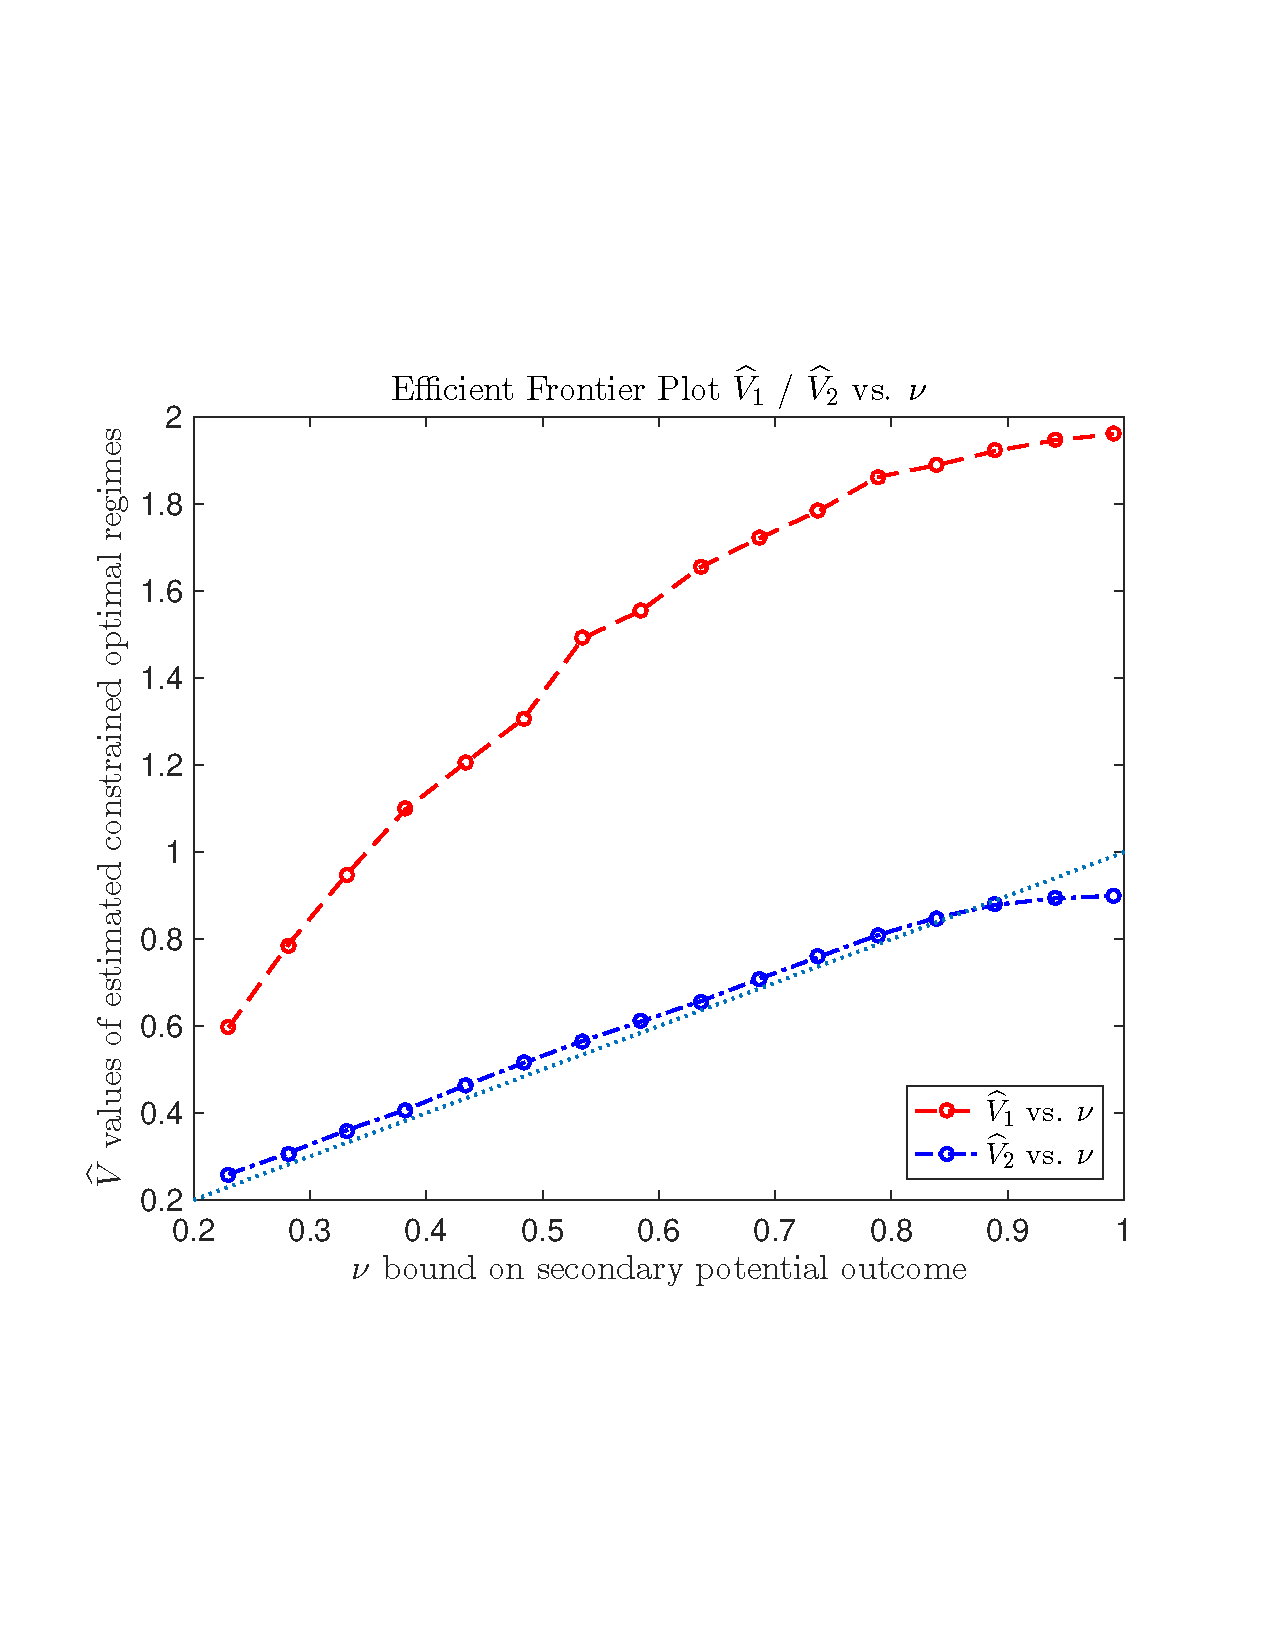
\includegraphics[width=\textwidth,height=\textheight,keepaspectratio]{/Users
/shuping.ruan/GitHub/thesis_research/Single-Stage-Constrained-Optimal
-Treatment-Regimes/ plot_results/efficient_plot1.pdf}
%    \caption{Probability distribution with loading level of a) 1.0 b) 1.1 }
%	\label{fig:1}
%\end{figure}	
%\end{frame}
%%%%----
%\begin{frame}
%\begin{table}[!htbp]
% \resizebox{\textwidth}{!}{
%	\centering
%	{\tt
%	
\begin{tabular}{rrrrrrrrrr}\hline 
$\nu$  & $\wh{V}_1(\wh{\bs{\theta}}_{\nu})$ & $std(\wh{V}_1)$ & $\wh{V}_2(\wh{\bs{\theta}}_{\nu})$ & $std(\wh{V}_2)$ & $\wh{\theta}_{\nu,1}$ & $std(\wh{\theta}_{\nu,1})$ & $\wh{\theta}_{\nu,2}$ & $std(\wh{\theta}_{\nu,2})$ \\ \hline 
%2 &      NaN &      NaN &      NaN  &      NaN &       NaN &       NaN &       NaN &       NaN &       NaN \\ 
%2 &      NaN &      NaN &      NaN  &      NaN &       NaN &       NaN &       NaN &       NaN &       NaN \\ 
%2 &    -2.99 &      NaN &      NaN  &      NaN &       NaN &       NaN &       NaN &       NaN &       NaN \\ 
-2.62 &     3.94 &     0.16  &    -2.61 &      0.10 &      0.14 &      0.07 &      0.99 &      0.01 \\ 
-2.26 &     4.32 &     0.07  &    -2.24 &      0.10 &     -0.06 &      0.05 &      1.00 &      0.00 \\ 
-1.89 &     4.48 &     0.03  &    -1.89 &      0.12 &     -0.22 &      0.04 &      0.98 &      0.01 \\ 
-1.52 &     4.54 &     0.01  &    -1.53 &      0.10 &     -0.35 &      0.04 &      0.94 &      0.01 \\ 
-1.16 &     4.55 &     0.00  &    -1.35 &      0.10 &     -0.41 &      0.04 &      0.91 &      0.02 \\ 
-0.79 &     4.55 &     0.00  &    -1.34 &      0.11 &     -0.42 &      0.04 &      0.91 &      0.02 \\ 
-0.42 &     4.55 &     0.00  &    -1.34 &      0.11 &     -0.42 &      0.04 &      0.91 &      0.02 \\ 
-0.06 &     4.55 &     0.00  &    -1.34 &      0.11 &     -0.42 &      0.04 &      0.91 &      0.02 \\ 
 0.31 &     4.55 &     0.00  &    -1.34 &      0.11 &     -0.42 &      0.04 &      0.91 &      0.02 \\ 
 0.68 &     4.55 &     0.00  &    -1.34 &      0.11 &     -0.42 &      0.04 &      0.91 &      0.02 \\ 
 1.04 &     4.55 &     0.00  &    -1.34 &      0.11 &     -0.42 &      0.04 &      0.91 &      0.02 \\ 
 1.41 &     4.55 &     0.00  &    -1.34 &      0.11 &     -0.42 &      0.04 &      0.91 &      0.02 \\ 
 1.78 &     4.55 &     0.00  &    -1.34 &      0.11 &     -0.42 &      0.04 &      0.91 &      0.02 \\ 
 2.14 &     4.55 &     0.00  &    -1.34 &      0.11 &     -0.42 &      0.04 &      0.91 &      0.02 \\ 
 2.51 &     4.55 &     0.00  &    -1.34 &      0.11 &     -0.42 &      0.04 &      0.91 &      0.02 \\ 
 2.88 &     4.55 &     0.00  &    -1.34 &      0.11 &     -0.42 &      0.04 &      0.91 &      0.02 \\ 
 3.24 &     4.55 &     0.00  &    -1.34 &      0.11 &     -0.42 &      0.04 &      0.91 &      0.02 \\ 
 3.61 &     4.44 &     0.89  &    -1.26 &      0.63 &     -0.41 &      0.04 &      0.88 &      0.23 \\ 
 3.97 &     4.55 &     0.00  &    -1.34 &      0.11 &     -0.42 &      0.04 &      0.91 &      0.02 \\ \hline 
\end{tabular}

%	}}
%\caption {Simulation Result for Setting 2}
%\end{table} 	
%\end{frame}
\begin{frame}
\begin{figure}	
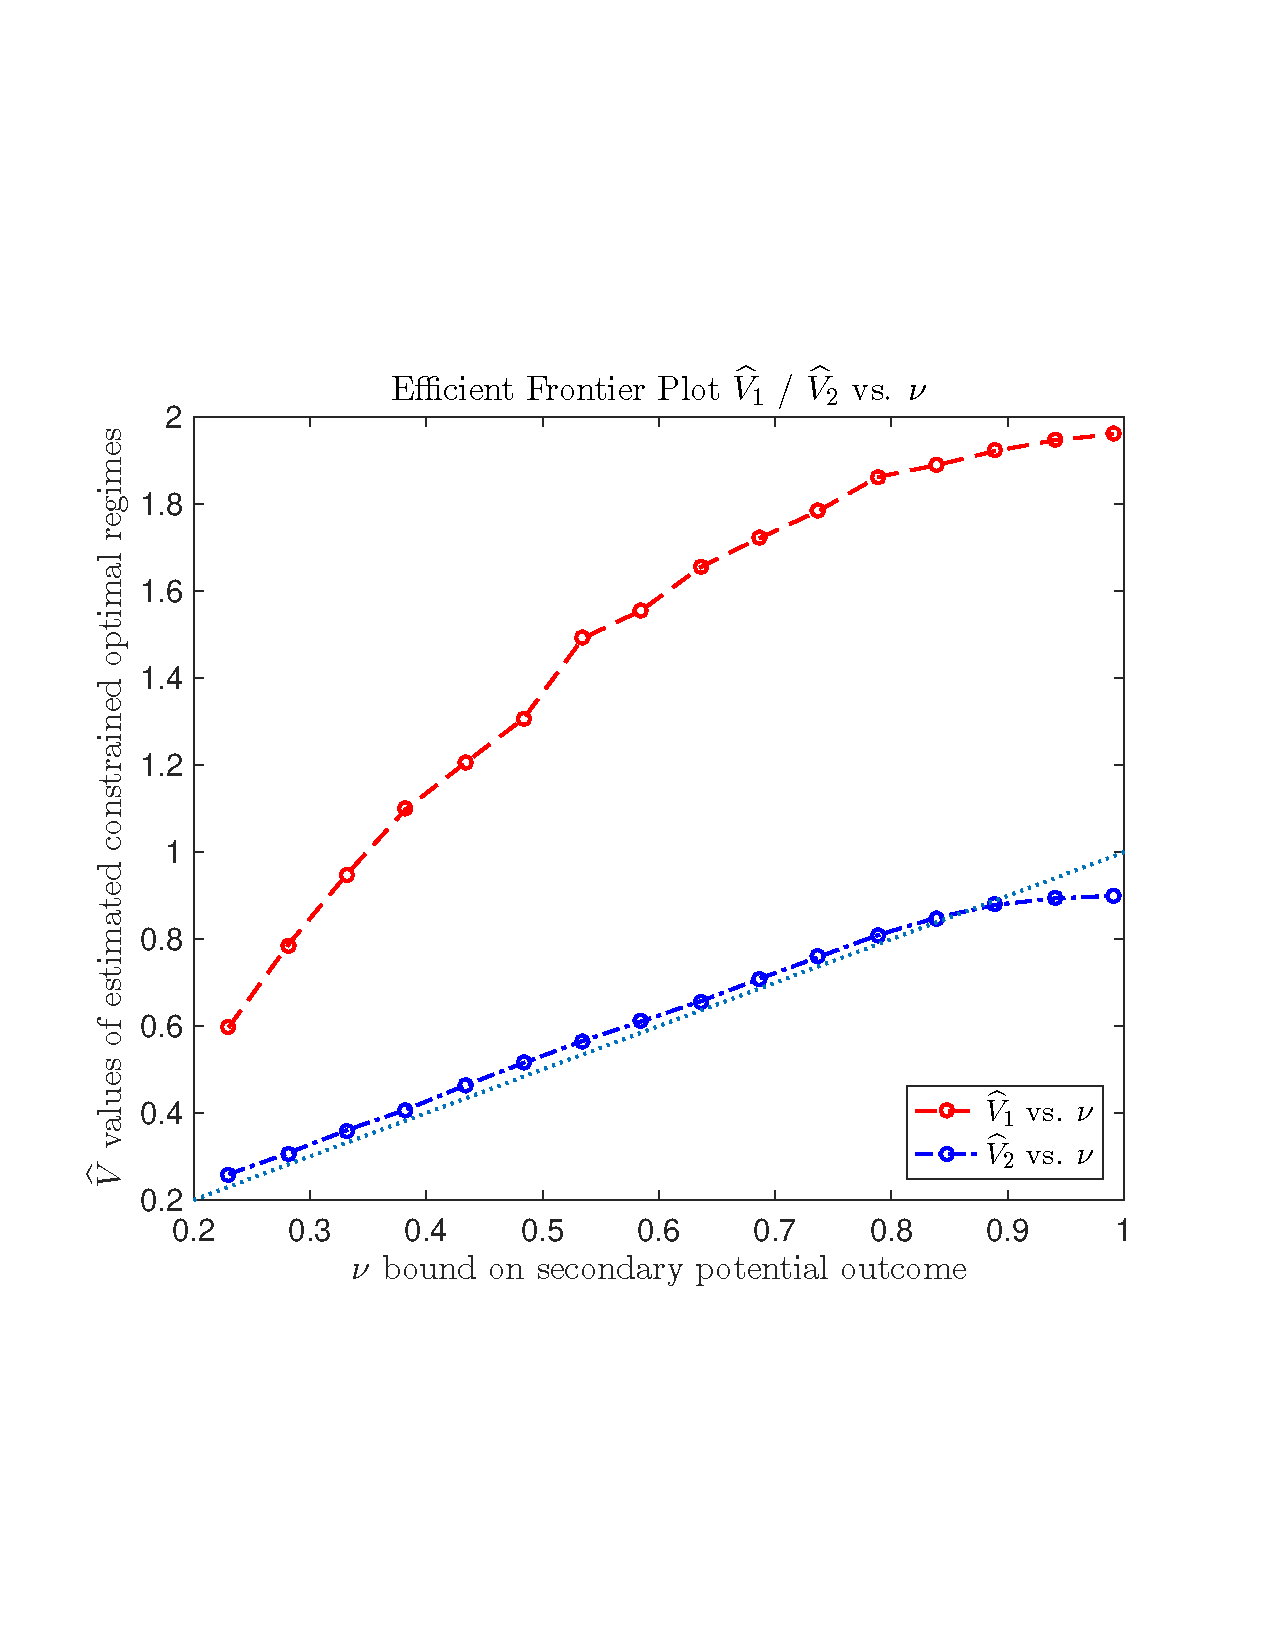
\includegraphics[width=\textwidth,height=\textheight,keepaspectratio]{/Users
/shuping.ruan/GitHub/thesis_research/Single-Stage-Constrained-Optimal
-Treatment-Regimes/plot_results/efficient_plot1.pdf}
	\caption{Efficient frontier for estimated constrained optimal regimes
(single-stage) for Setting 1.}
	\label{fig:1}
\end{figure}	
\end{frame}
%%%----
%\begin{frame}
%\begin{table}[!htbp]
% \resizebox{\textwidth}{!}{
%	\centering
%	{\tt
%	
\begin{tabular}{rrrrrrrrrr}\hline 
$\nu$  & $\wh{V}_1(\wh{\bs{\theta}}_{\nu})$ & $std(\wh{V}_1)$ & $\wh{V}_2(\wh{\bs{\theta}}_{\nu})$ & $std(\wh{V}_2)$ & $\wh{\theta}_{\nu,1}$ & $std(\wh{\theta}_{\nu,1})$ & $\wh{\theta}_{\nu,2}$ & $std(\wh{\theta}_{\nu,2})$ \\ \hline 
-2.50 &     1.19 &     0.19  &    -2.55 &      0.15 &     -0.05 &      0.10 &      0.99 &      0.01 \\ 
-2.15 &     1.33 &     0.05  &    -2.18 &      0.16 &     -0.24 &      0.07 &      0.97 &      0.02 \\ 
-1.80 &     1.42 &     0.04  &    -1.82 &      0.17 &     -0.39 &      0.06 &      0.92 &      0.03 \\ 
-1.45 &     1.50 &     0.04  &    -1.48 &      0.17 &     -0.51 &      0.06 &      0.86 &      0.03 \\ 
-1.09 &     1.56 &     0.03  &    -1.15 &      0.18 &     -0.60 &      0.05 &      0.79 &      0.04 \\ 
-0.74 &     1.61 &     0.02  &    -0.83 &      0.20 &     -0.69 &      0.05 &      0.72 &      0.04 \\ 
-0.39 &     1.62 &     0.02  &    -0.53 &      0.26 &     -0.75 &      0.06 &      0.66 &      0.06 \\ 
-0.04 &     1.63 &     0.01  &    -0.30 &      0.32 &     -0.79 &      0.06 &      0.61 &      0.07 \\ 
 0.32 &     1.63 &     0.01  &    -0.18 &      0.43 &     -0.81 &      0.07 &      0.58 &      0.10 \\ 
 0.67 &     1.63 &     0.01  &    -0.06 &      0.47 &     -0.82 &      0.08 &      0.55 &      0.11 \\ 
 1.02 &     1.63 &     0.01  &    -0.08 &      0.51 &     -0.82 &      0.08 &      0.55 &      0.12 \\ 
 1.37 &     1.63 &     0.01  &    -0.03 &      0.52 &     -0.83 &      0.08 &      0.54 &      0.13 \\ 
 1.73 &     1.62 &     0.02  &    -0.04 &      0.53 &     -0.83 &      0.08 &      0.54 &      0.13 \\ 
 2.08 &     1.63 &     0.01  &    -0.04 &      0.50 &     -0.83 &      0.08 &      0.54 &      0.12 \\ 
 2.43 &     1.63 &     0.01  &    -0.03 &      0.51 &     -0.83 &      0.08 &      0.54 &      0.12 \\ 
 2.78 &     1.63 &     0.01  &    -0.03 &      0.51 &     -0.83 &      0.08 &      0.54 &      0.12 \\ 
 3.13 &     1.63 &     0.01  &    -0.02 &      0.50 &     -0.83 &      0.08 &      0.54 &      0.12 \\ 
 3.49 &     1.62 &     0.13  &     0.01 &      0.57 &     -0.83 &      0.10 &      0.53 &      0.17 \\ 
 3.84 &     1.63 &     0.01  &     0.00 &      0.52 &     -0.83 &      0.08 &      0.53 &      0.13 \\ \hline 
\end{tabular}

%	}}
%\caption {Simulation Result for Setting 3}
%\end{table} 	
%\end{frame}
%\begin{frame}
%\begin{figure}
%
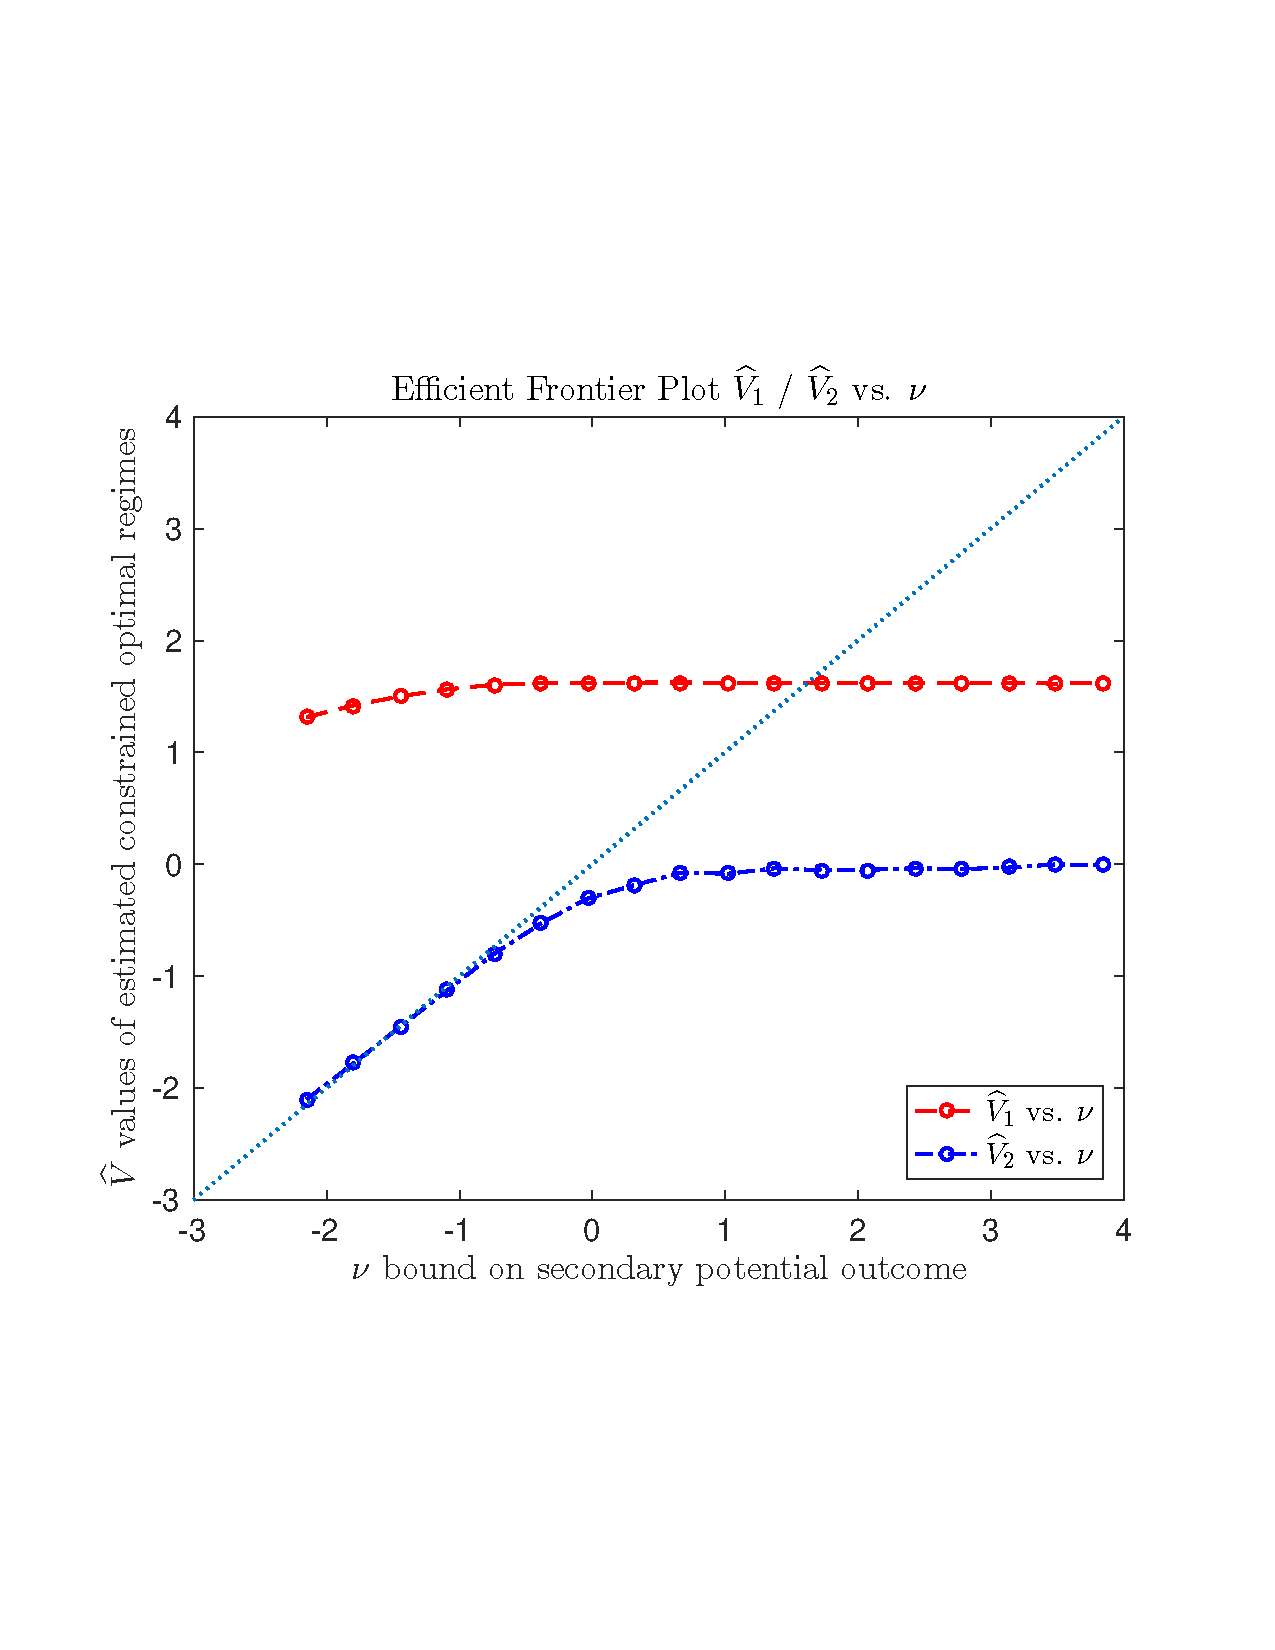
\includegraphics[width=\textwidth,height=\textheight,keepaspectratio]{//Users
/shuping.ruan/GitHub/thesis_research/Single-Stage-Constrained-Optimal
-Treatment-Regimes/plot_results/efficient_plot3.pdf}
%	\caption{Efficient frontier for estimated constrained optimal regimes
(single-stage) for Setting 3.}
%	\label{fig:3}
%\end{figure}	
%\end{frame}
%%%---
%\begin{frame}
%\begin{table}[!htbp]
% \resizebox{\textwidth}{!}{
%	\centering
%	{\tt
%	
\begin{tabular}{rrrrrrrrrr}\hline 
$\nu$  & $\wh{V}_1(\wh{\bs{\theta}}_{\nu})$ & $std(\wh{V}_1)$ & $\wh{V}_2(\wh{\bs{\theta}}_{\nu})$ & $std(\wh{V}_2)$ & $\wh{\theta}_{\nu,1}$ & $std(\wh{\theta}_{\nu,1})$ & $\wh{\theta}_{\nu,2}$ & $std(\wh{\theta}_{\nu,2})$ \\ \hline 
%4 &      NaN &      NaN &      NaN  &      NaN &       NaN &       NaN &       NaN &       NaN &       NaN \\ 
%4 &      NaN &      NaN &      NaN  &      NaN &       NaN &       NaN &       NaN &       NaN &       NaN \\ 
%4 &    -1.81 &      NaN &      NaN  &      NaN &       NaN &       NaN &       NaN &       NaN &       NaN \\ 
-1.57 &     1.62 &     0.01  &    -1.82 &      0.03 &      0.14 &      0.12 &     -0.98 &      0.02 \\ 
-1.32 &     1.62 &     0.02  &    -1.81 &      0.04 &      0.14 &      0.13 &     -0.98 &      0.02 \\ 
-1.08 &     1.62 &     0.02  &    -1.82 &      0.03 &      0.15 &      0.13 &     -0.98 &      0.02 \\ 
-0.84 &     1.62 &     0.02  &    -1.81 &      0.04 &      0.14 &      0.13 &     -0.98 &      0.02 \\ 
-0.59 &     1.62 &     0.02  &    -1.81 &      0.04 &      0.14 &      0.13 &     -0.98 &      0.02 \\ 
-0.35 &     1.62 &     0.02  &    -1.81 &      0.04 &      0.14 &      0.13 &     -0.98 &      0.02 \\ 
-0.10 &     1.62 &     0.02  &    -1.81 &      0.04 &      0.14 &      0.13 &     -0.98 &      0.02 \\ 
 0.14 &     1.62 &     0.02  &    -1.81 &      0.04 &      0.14 &      0.13 &     -0.98 &      0.02 \\ 
 0.38 &     1.62 &     0.02  &    -1.81 &      0.04 &      0.14 &      0.13 &     -0.98 &      0.02 \\ 
 0.63 &     1.62 &     0.02  &    -1.81 &      0.04 &      0.14 &      0.13 &     -0.98 &      0.02 \\ 
 0.87 &     1.62 &     0.02  &    -1.81 &      0.04 &      0.14 &      0.14 &     -0.98 &      0.02 \\ 
 1.11 &     1.62 &     0.02  &    -1.81 &      0.04 &      0.14 &      0.13 &     -0.98 &      0.02 \\ 
 1.36 &     1.62 &     0.02  &    -1.81 &      0.04 &      0.15 &      0.13 &     -0.98 &      0.02 \\ 
 1.60 &     1.62 &     0.02  &    -1.81 &      0.04 &      0.14 &      0.13 &     -0.98 &      0.02 \\ 
 1.84 &     1.62 &     0.02  &    -1.81 &      0.04 &      0.14 &      0.13 &     -0.98 &      0.02 \\ 
 2.09 &     1.62 &     0.02  &    -1.81 &      0.04 &      0.14 &      0.13 &     -0.98 &      0.02 \\ 
 2.33 &     1.62 &     0.02  &    -1.81 &      0.04 &      0.14 &      0.13 &     -0.98 &      0.02 \\ 
 2.57 &     1.62 &     0.02  &    -1.81 &      0.04 &      0.14 &      0.13 &     -0.98 &      0.02 \\ 
 2.82 &     1.62 &     0.02  &    -1.81 &      0.04 &      0.14 &      0.13 &     -0.98 &      0.02 \\ \hline 
\end{tabular}

%	}}
%\caption {Simulation Result for Setting 4}
%\end{table} 	
%\end{frame}
%\begin{frame}
%\begin{figure}
%
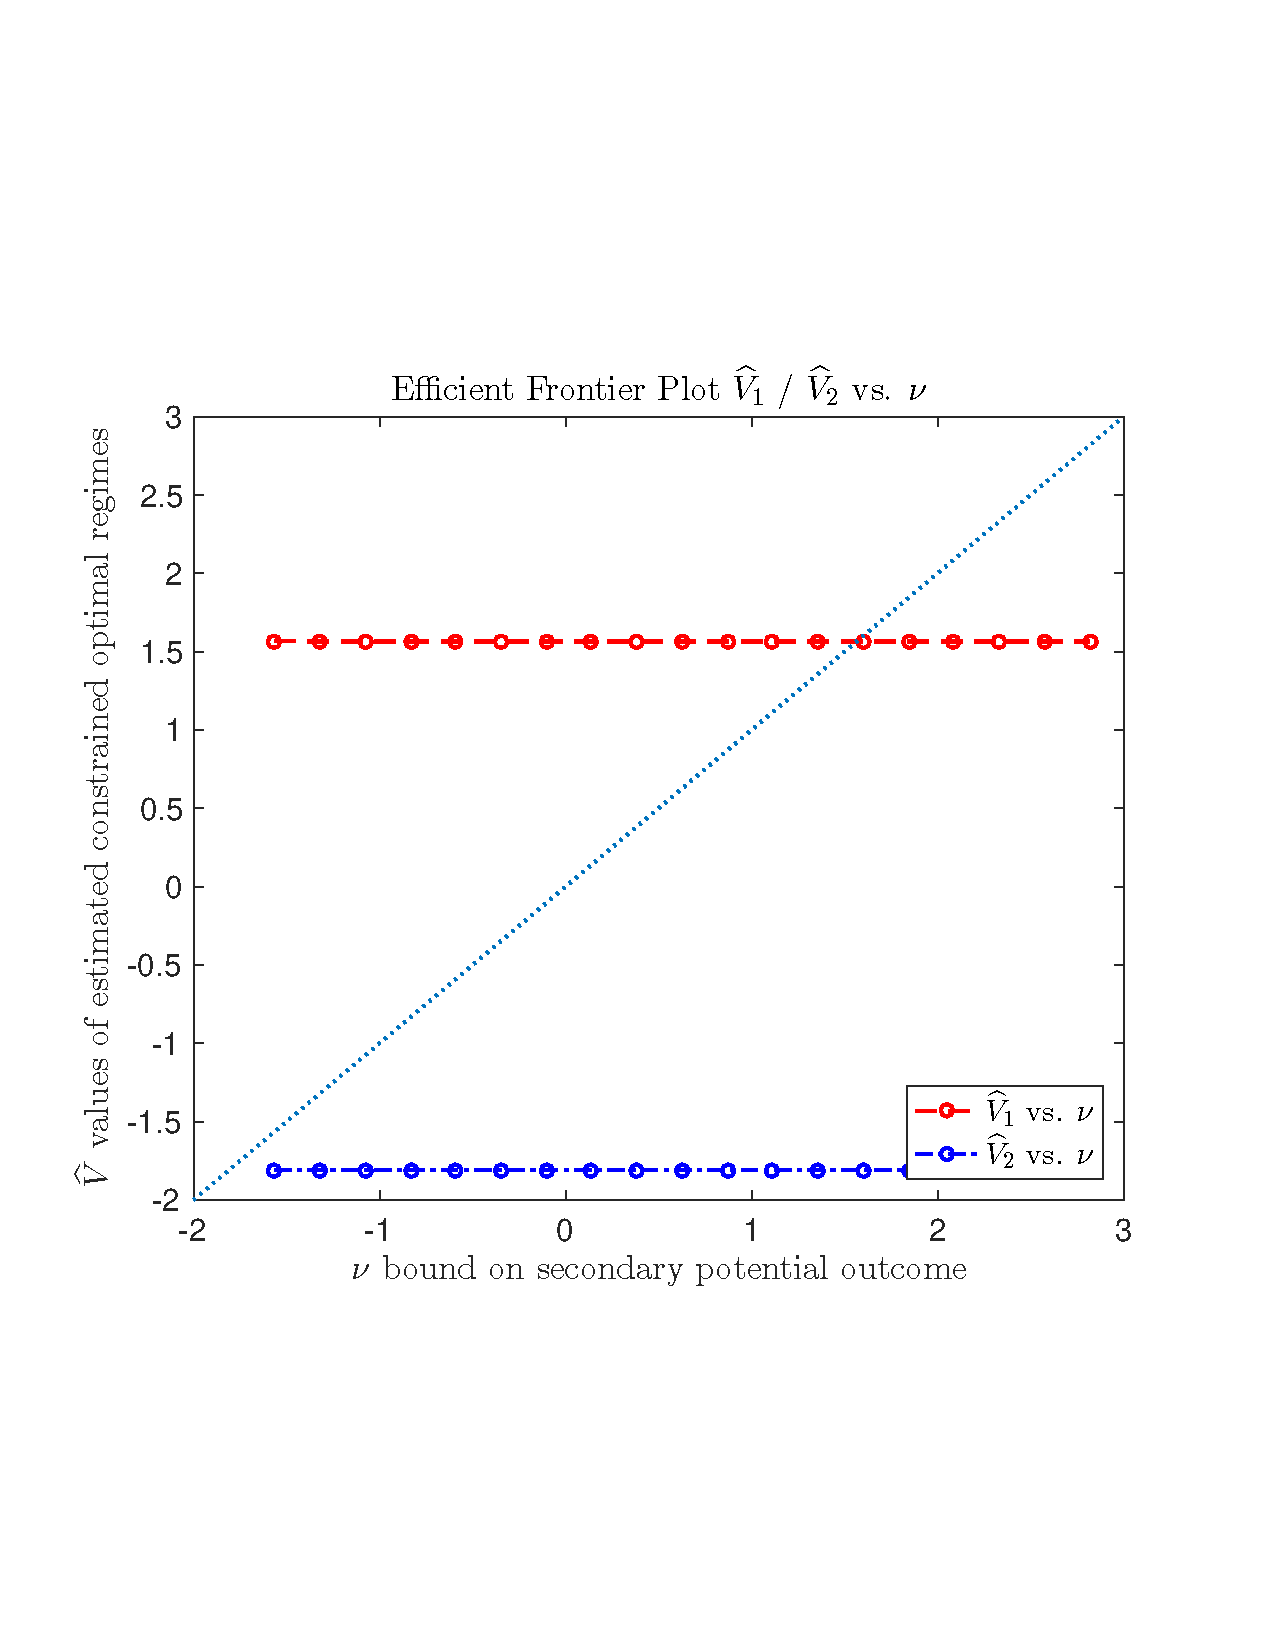
\includegraphics[width=\textwidth,height=\textheight,keepaspectratio]{//Users
/shuping.ruan/GitHub/thesis_research/Single-Stage-Constrained-Optimal
-Treatment-Regimes/plot_results/efficient_plot4.pdf}
%	\caption{Efficient frontier for estimated constrained optimal regimes
(single-stage) for Setting 4.}
%	\label{fig:4}
%\end{figure}	
%\end{frame}
%%---
%\begin{frame}
%\begin{table}[!htbp]
% \resizebox{\textwidth}{!}{
%	\centering
%	{\tt
%	
\begin{tabular}{rrrrrrrrrr}\hline 
$\nu$  & $\wh{V}_1(\wh{\bs{\theta}}_{\nu})$ & $std(\wh{V}_1)$ & $\wh{V}_2(\wh{\bs{\theta}}_{\nu})$ & $std(\wh{V}_2)$ & $\wh{\theta}_{\nu,1}$ & $std(\wh{\theta}_{\nu,1})$ & $\wh{\theta}_{\nu,2}$ & $std(\wh{\theta}_{\nu,2})$ \\ \hline 
%5 &      NaN &      NaN &      NaN  &      NaN &       NaN &       NaN &       NaN &       NaN &       NaN \\ 
%5 &      NaN &      NaN &      NaN  &      NaN &       NaN &       NaN &       NaN &       NaN &       NaN \\ 
%5 &    -2.94 &      NaN &      NaN  &      NaN &       NaN &       NaN &       NaN &       NaN &       NaN \\ 
-2.58 &     0.64 &     0.04  &    -2.62 &      0.15 &      0.80 &      0.09 &     -0.59 &      0.10 \\ 
-2.22 &     0.70 &     0.03  &    -2.29 &      0.20 &      0.90 &      0.07 &     -0.42 &      0.11 \\ 
-1.85 &     0.74 &     0.04  &    -1.97 &      0.24 &      0.95 &      0.07 &     -0.27 &      0.12 \\ 
-1.49 &     0.76 &     0.04  &    -1.68 &      0.33 &      0.98 &      0.05 &     -0.16 &      0.14 \\ 
-1.13 &     0.79 &     0.04  &    -1.37 &      0.39 &      0.99 &      0.04 &     -0.05 &      0.15 \\ 
-0.77 &     0.80 &     0.04  &    -1.12 &      0.46 &      0.98 &      0.03 &      0.04 &      0.17 \\ 
-0.40 &     0.80 &     0.05  &    -0.91 &      0.59 &      0.97 &      0.06 &      0.10 &      0.22 \\ 
-0.04 &     0.80 &     0.05  &    -0.67 &      0.63 &      0.95 &      0.13 &      0.18 &      0.22 \\ 
 0.32 &     0.80 &     0.06  &    -0.44 &      0.75 &      0.92 &      0.15 &      0.24 &      0.27 \\ 
 0.68 &     0.80 &     0.06  &    -0.23 &      0.82 &      0.91 &      0.15 &      0.29 &      0.26 \\ 
 1.05 &     0.80 &     0.07  &    -0.08 &      0.93 &      0.88 &      0.19 &      0.33 &      0.28 \\ 
 1.41 &     0.80 &     0.07  &     0.10 &      0.97 &      0.86 &      0.20 &      0.37 &      0.28 \\ 
 1.77 &     0.80 &     0.05  &     0.15 &      1.04 &      0.86 &      0.17 &      0.39 &      0.29 \\ 
 2.13 &     0.80 &     0.05  &     0.24 &      1.10 &      0.84 &      0.18 &      0.41 &      0.30 \\ 
 2.50 &     0.80 &     0.05  &     0.29 &      1.14 &      0.83 &      0.19 &      0.42 &      0.31 \\ 
 2.86 &     0.80 &     0.03  &     0.38 &      1.20 &      0.82 &      0.17 &      0.44 &      0.31 \\ 
 3.22 &     0.80 &     0.03  &     0.44 &      1.21 &      0.81 &      0.19 &      0.46 &      0.31 \\ 
 3.58 &     0.80 &     0.03  &     0.34 &      1.19 &      0.83 &      0.18 &      0.44 &      0.31 \\ 
 3.94 &     0.80 &     0.04  &     0.48 &      1.29 &      0.80 &      0.22 &      0.46 &      0.32 \\ \hline 
\end{tabular}

%	}}
%\caption {Simulation Result for Setting 5}
%\end{table} 	
%\end{frame}
%\begin{frame}
%\begin{figure}
%
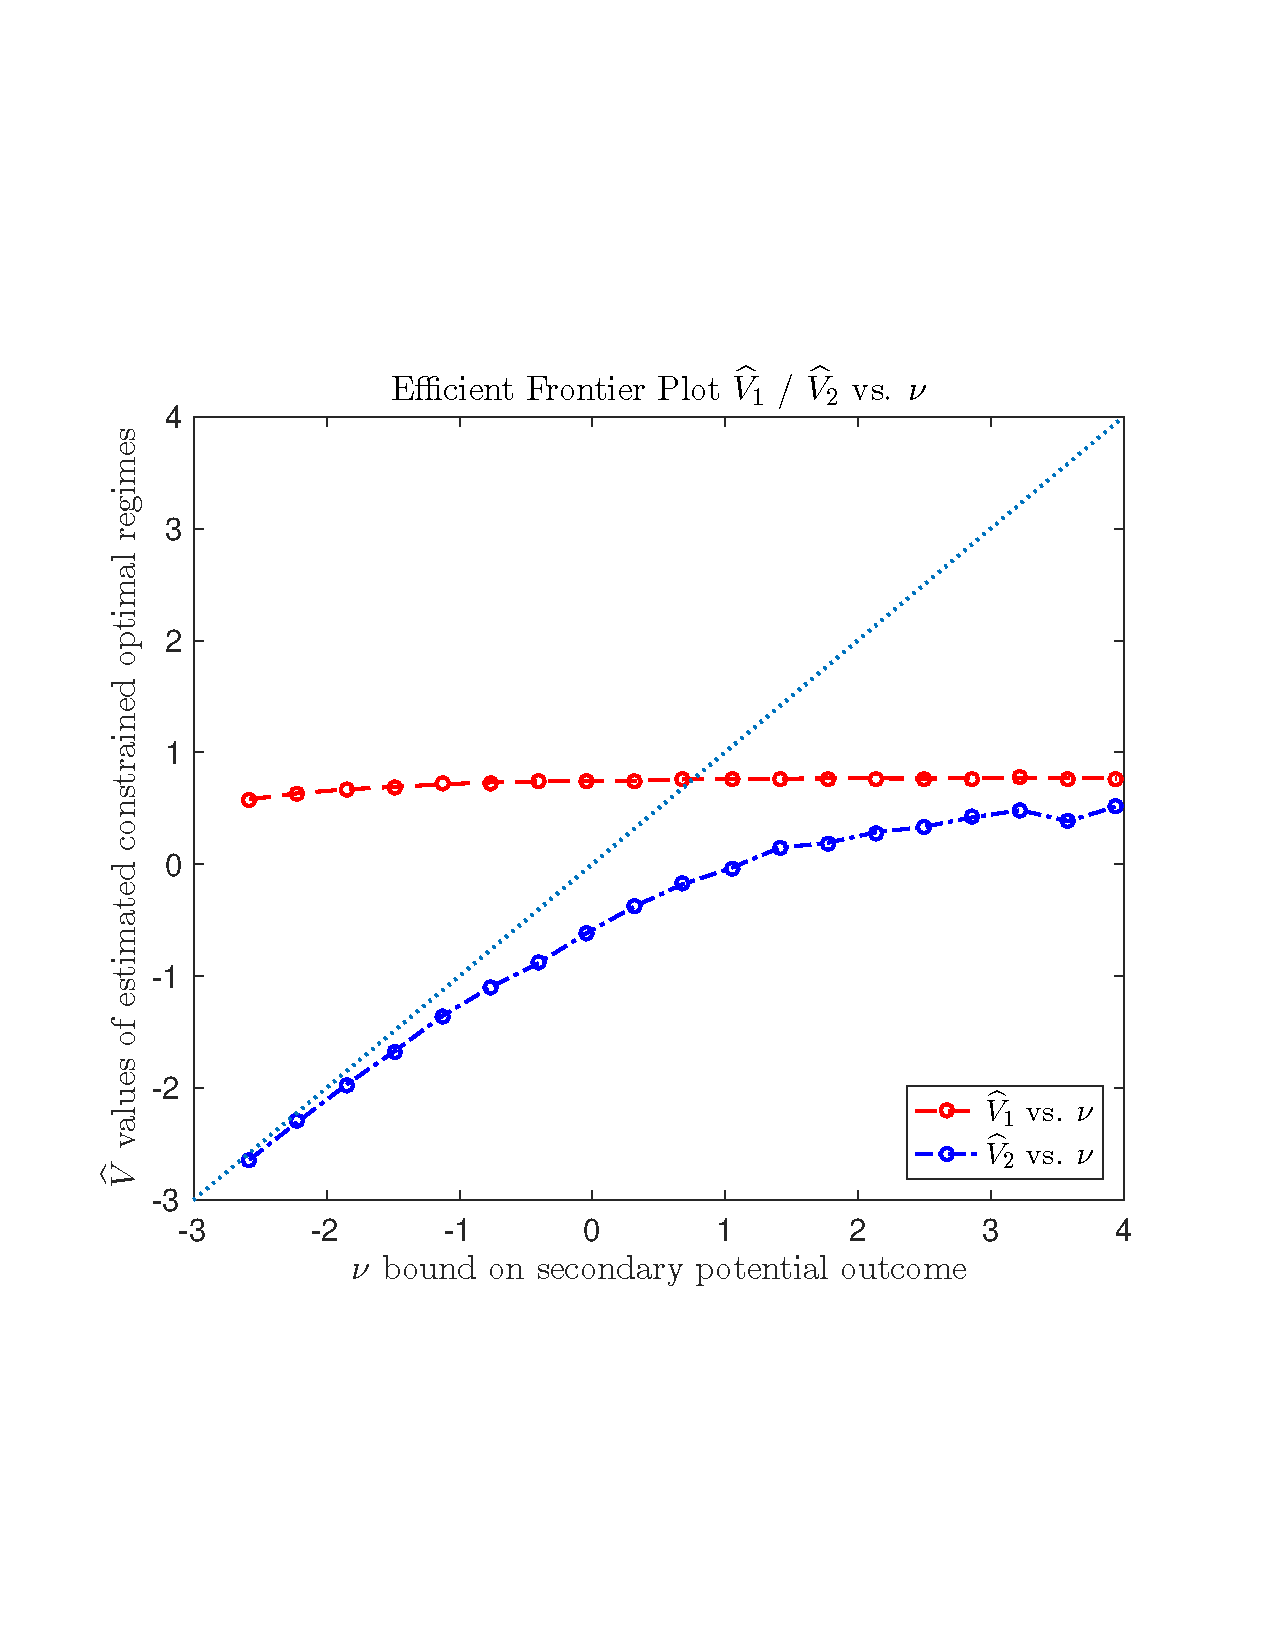
\includegraphics[width=\textwidth,height=\textheight,keepaspectratio]{//Users
/shuping.ruan/GitHub/thesis_research/Single-Stage-Constrained-Optimal
-Treatment-Regimes/plot_results/efficient_plot5.pdf}
%	\caption{Efficient frontier for estimated constrained optimal regimes
(single-stage) for Setting 5.}
%	\label{fig:5}
%\end{figure}	
%\end{frame}
%%%--
%%%---
%\begin{frame}
%\begin{table}[!htbp]
% \resizebox{\textwidth}{!}{
%	\centering
%	{\tt
%	
\begin{tabular}{rrrrrrrrrr}\hline 
$\nu$  & $\wh{V}_1(\wh{\bs{\theta}}_{\nu})$ & $std(\wh{V}_1)$ & $\wh{V}_2(\wh{\bs{\theta}}_{\nu})$ & $std(\wh{V}_2)$ & $\wh{\theta}_{\nu,1}$ & $std(\wh{\theta}_{\nu,1})$ & $\wh{\theta}_{\nu,2}$ & $std(\wh{\theta}_{\nu,2})$ \\ \hline 
%6 &      NaN &      NaN &      NaN  &      NaN &       NaN &       NaN &       NaN &       NaN &       NaN \\ 
%6 &      NaN &      NaN &      NaN  &      NaN &       NaN &       NaN &       NaN &       NaN &       NaN \\ 
%6 &    -0.61 &      NaN &      NaN  &      NaN &       NaN &       NaN &       NaN &       NaN &       NaN \\ 
-0.50 &     0.59 &     0.11  &    -0.55 &      0.41 &     -0.83 &      0.31 &     -0.44 &      0.13 \\ 
-0.38 &     0.73 &     0.08  &    -0.36 &      0.07 &     -0.96 &      0.03 &     -0.26 &      0.11 \\ 
-0.26 &     0.85 &     0.07  &    -0.25 &      0.08 &     -0.99 &      0.01 &     -0.11 &      0.10 \\ 
-0.14 &     0.94 &     0.06  &    -0.13 &      0.09 &     -1.00 &      0.01 &      0.02 &      0.09 \\ 
-0.03 &     1.01 &     0.05  &    -0.00 &      0.09 &     -0.99 &      0.01 &      0.15 &      0.08 \\ 
 0.09 &     1.07 &     0.04  &     0.12 &      0.09 &     -0.96 &      0.02 &      0.26 &      0.08 \\ 
 0.21 &     1.12 &     0.03  &     0.24 &      0.09 &     -0.93 &      0.03 &      0.36 &      0.07 \\ 
 0.33 &     1.15 &     0.14  &     0.36 &      0.09 &     -0.87 &      0.17 &      0.45 &      0.13 \\ 
 0.44 &     1.18 &     0.14  &     0.48 &      0.08 &     -0.82 &      0.17 &      0.54 &      0.13 \\ 
 0.56 &     1.21 &     0.14  &     0.60 &      0.09 &     -0.76 &      0.17 &      0.62 &      0.13 \\ 
 0.68 &     1.20 &     0.25  &     0.71 &      0.09 &     -0.65 &      0.30 &      0.67 &      0.22 \\ 
 0.80 &     1.23 &     0.19  &     0.80 &      0.09 &     -0.61 &      0.23 &      0.74 &      0.17 \\ 
 0.91 &     1.23 &     0.18  &     0.88 &      0.10 &     -0.56 &      0.23 &      0.78 &      0.16 \\ 
 1.03 &     1.25 &     0.09  &     0.92 &      0.12 &     -0.54 &      0.15 &      0.82 &      0.10 \\ 
 1.15 &     1.26 &     0.01  &     0.95 &      0.14 &     -0.52 &      0.12 &      0.84 &      0.08 \\ 
 1.27 &     1.25 &     0.01  &     0.96 &      0.15 &     -0.51 &      0.13 &      0.85 &      0.08 \\ 
 1.38 &     1.25 &     0.01  &     0.96 &      0.15 &     -0.51 &      0.12 &      0.85 &      0.08 \\ 
 1.50 &     1.25 &     0.01  &     0.96 &      0.15 &     -0.51 &      0.13 &      0.85 &      0.08 \\ 
 1.62 &     1.25 &     0.01  &     0.96 &      0.15 &     -0.51 &      0.13 &      0.85 &      0.08 \\ \hline 
\end{tabular}

%	}}
%\caption {Simulation Result for Setting 6}
%\end{table} 	
%\end{frame}
%\begin{frame}
%\begin{figure}
%
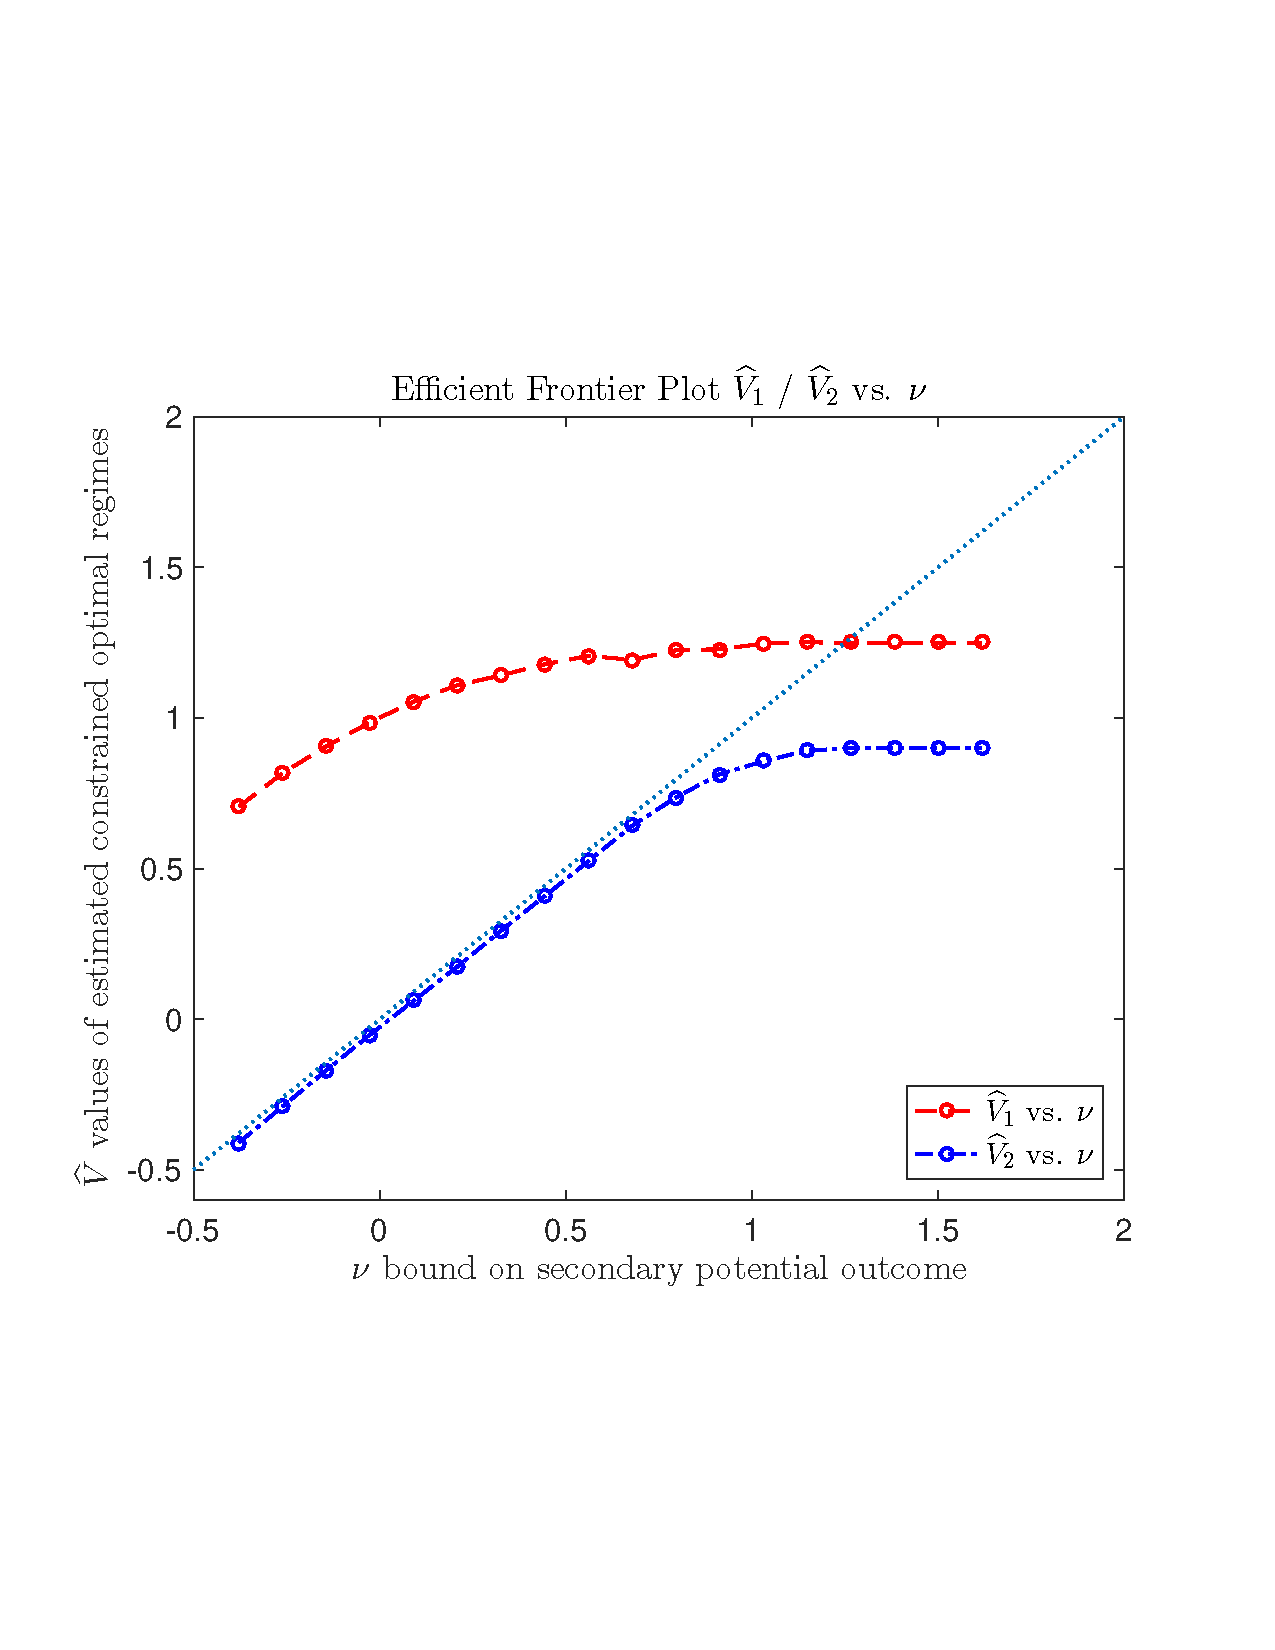
\includegraphics[width=\textwidth,height=\textheight,keepaspectratio]{//Users
/shuping.ruan/GitHub/thesis_research/Single-Stage-Constrained-Optimal
-Treatment-Regimes/plot_results/efficient_plot6.pdf}
%	\caption{Efficient frontier for estimated constrained optimal regimes
(single-stage) for Setting 6.}
%	\label{fig:6}
%\end{figure}	
%\end{frame}
%%%--
%%%---
%\begin{frame}
%\begin{table}[!htbp]
% \resizebox{\textwidth}{!}{
%	\centering
%	{\tt
%	
\begin{tabular}{rrrrrrrrrr}\hline 
$\nu$  & $\wh{V}_1(\wh{\bs{\theta}}_{\nu})$ & $std(\wh{V}_1)$ & $\wh{V}_2(\wh{\bs{\theta}}_{\nu})$ & $std(\wh{V}_2)$ & $\wh{\theta}_{\nu,1}$ & $std(\wh{\theta}_{\nu,1})$ & $\wh{\theta}_{\nu,2}$ & $std(\wh{\theta}_{\nu,2})$ \\ \hline 
%7 &      NaN &      NaN &      NaN  &      NaN &       NaN &       NaN &       NaN &       NaN &       NaN \\ 
%7 &      NaN &      NaN &      NaN  &      NaN &       NaN &       NaN &       NaN &       NaN &       NaN \\ 
%7 &    -3.42 &      NaN &      NaN  &      NaN &       NaN &       NaN &       NaN &       NaN &       NaN \\ 
-3.01 &     1.12 &     0.01  &    -3.28 &      0.12 &     -0.70 &      0.10 &      0.70 &      0.10 \\ 
-2.60 &     1.12 &     0.01  &    -3.27 &      0.14 &     -0.69 &      0.11 &      0.71 &      0.10 \\ 
-2.19 &     1.12 &     0.01  &    -3.26 &      0.16 &     -0.69 &      0.11 &      0.71 &      0.11 \\ 
-1.77 &     1.12 &     0.01  &    -3.26 &      0.17 &     -0.69 &      0.11 &      0.71 &      0.11 \\ 
-1.36 &     1.12 &     0.01  &    -3.27 &      0.14 &     -0.69 &      0.11 &      0.70 &      0.11 \\ 
-0.95 &     1.12 &     0.01  &    -3.26 &      0.17 &     -0.69 &      0.11 &      0.71 &      0.11 \\ 
-0.54 &     1.12 &     0.01  &    -3.26 &      0.17 &     -0.69 &      0.11 &      0.71 &      0.11 \\ 
-0.12 &     1.12 &     0.01  &    -3.26 &      0.17 &     -0.69 &      0.11 &      0.71 &      0.11 \\ 
 0.29 &     1.12 &     0.01  &    -3.25 &      0.17 &     -0.69 &      0.11 &      0.71 &      0.11 \\ 
 0.70 &     1.12 &     0.01  &    -3.26 &      0.17 &     -0.69 &      0.12 &      0.71 &      0.11 \\ 
 1.11 &     1.12 &     0.01  &    -3.25 &      0.17 &     -0.68 &      0.11 &      0.71 &      0.11 \\ 
 1.53 &     1.12 &     0.01  &    -3.26 &      0.17 &     -0.69 &      0.11 &      0.71 &      0.11 \\ 
 1.94 &     1.12 &     0.01  &    -3.26 &      0.17 &     -0.69 &      0.11 &      0.71 &      0.11 \\ 
 2.35 &     1.12 &     0.01  &    -3.26 &      0.17 &     -0.69 &      0.11 &      0.71 &      0.11 \\ 
 2.76 &     1.12 &     0.01  &    -3.26 &      0.17 &     -0.69 &      0.11 &      0.71 &      0.11 \\ 
 3.18 &     1.12 &     0.01  &    -3.26 &      0.17 &     -0.69 &      0.11 &      0.71 &      0.11 \\ 
 3.59 &     1.12 &     0.01  &    -3.25 &      0.17 &     -0.68 &      0.11 &      0.71 &      0.11 \\ 
 4.00 &     1.12 &     0.01  &    -3.25 &      0.17 &     -0.69 &      0.11 &      0.71 &      0.11 \\ 
 4.41 &     1.11 &     0.08  &    -3.22 &      0.57 &     -0.68 &      0.15 &      0.70 &      0.14 \\ \hline 
\end{tabular}

%	}}
%\caption {Simulation Result for Setting 7}
%\end{table} 	
%\end{frame}
%\begin{frame}
%\begin{figure}
%
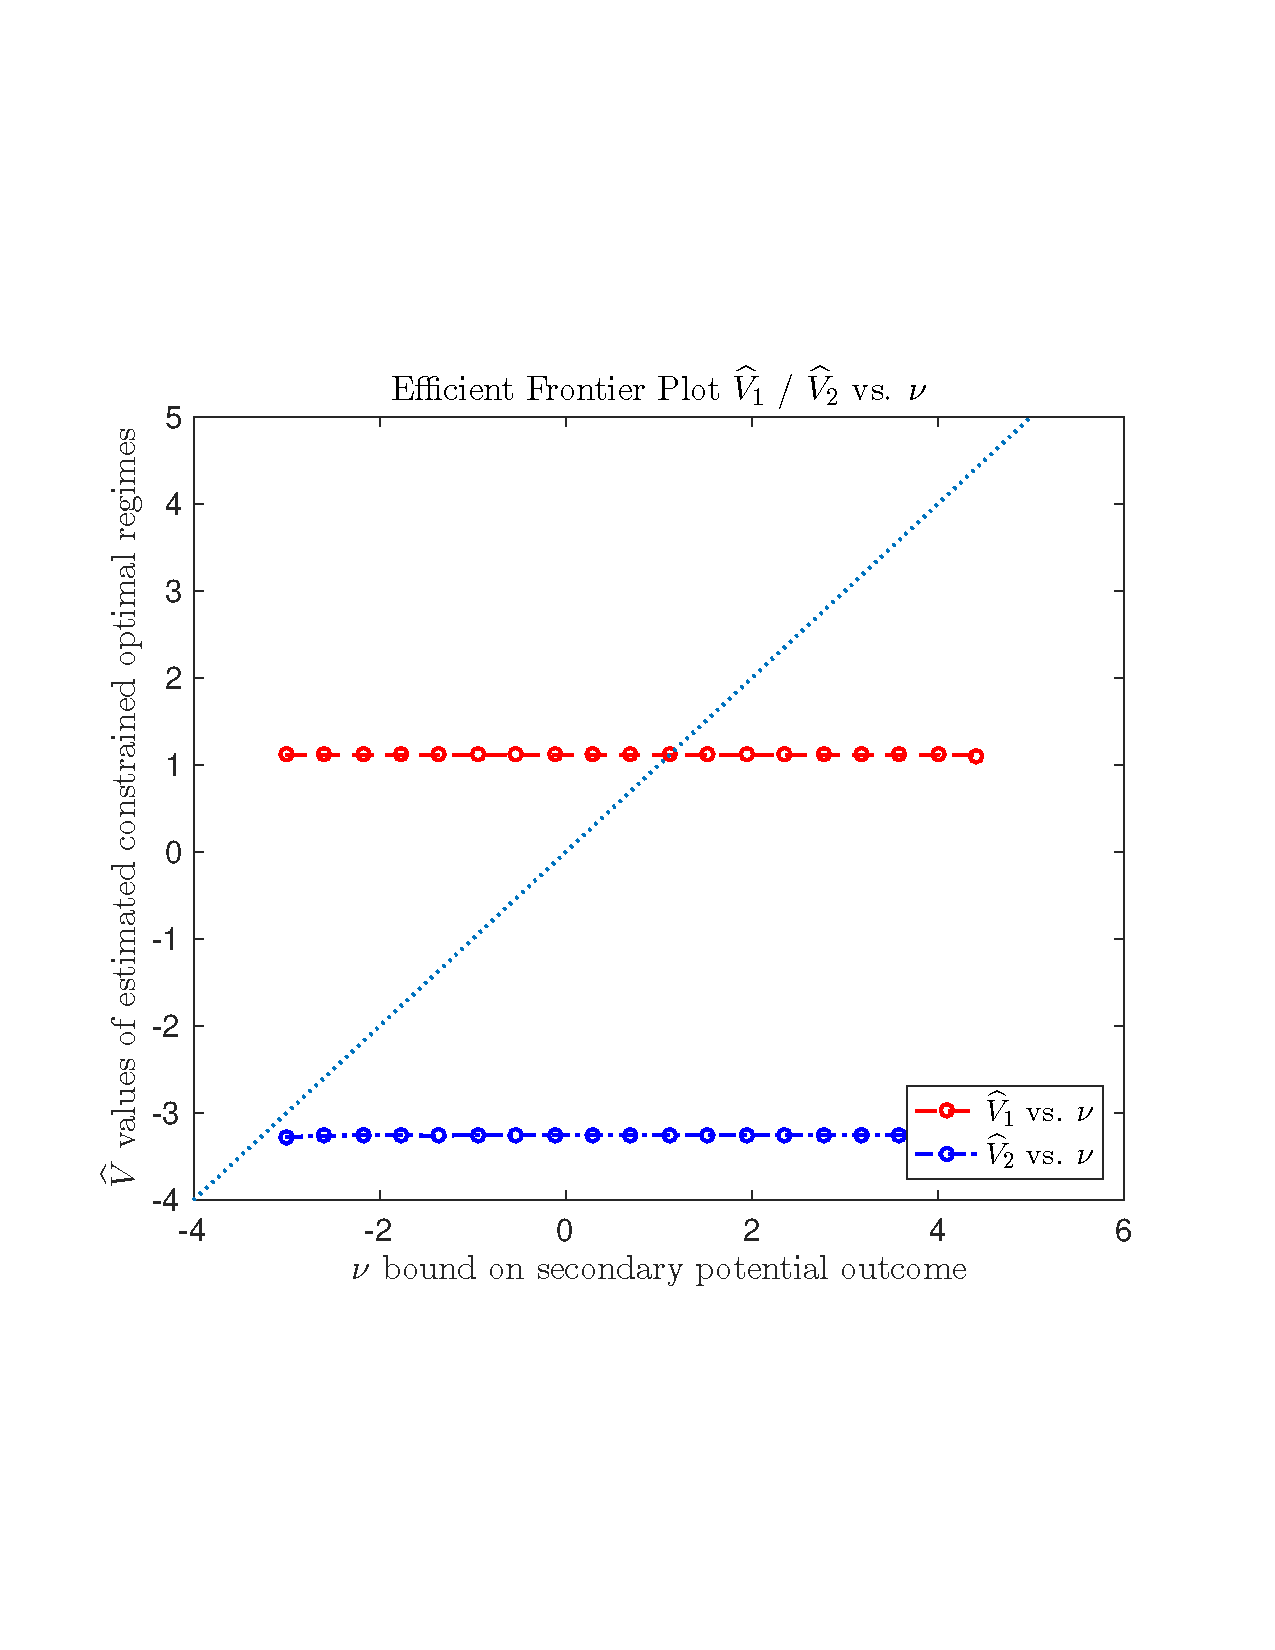
\includegraphics[width=\textwidth,height=\textheight,keepaspectratio]{//Users
/shuping.ruan/GitHub/thesis_research/Single-Stage-Constrained-Optimal
-Treatment-Regimes/plot_results/efficient_plot7.pdf}
%	\caption{Efficient frontier for estimated constrained optimal regimes
(single-stage) for Setting 7.}
%	\label{fig:7}
%\end{figure}	
%\end{frame}
%%%--
%%%---
%\begin{frame}
%\begin{table}[!htbp]
% \resizebox{\textwidth}{!}{
%	\centering
%	{\tt
%	
\begin{tabular}{rrrrrrrrrr}\hline 
$\nu$  & $\wh{V}_1(\wh{\bs{\theta}}_{\nu})$ & $std(\wh{V}_1)$ & $\wh{V}_2(\wh{\bs{\theta}}_{\nu})$ & $std(\wh{V}_2)$ & $\wh{\theta}_{\nu,1}$ & $std(\wh{\theta}_{\nu,1})$ & $\wh{\theta}_{\nu,2}$ & $std(\wh{\theta}_{\nu,2})$ \\ \hline 
%8 &      NaN &      NaN &      NaN  &      NaN &       NaN &       NaN &       NaN &       NaN &       NaN \\ 
%8 &      NaN &      NaN &      NaN  &      NaN &       NaN &       NaN &       NaN &       NaN &       NaN \\ 
%8 &    -3.19 &      NaN &      NaN  &      NaN &       NaN &       NaN &       NaN &       NaN &       NaN \\ 
-2.80 &    -0.36 &     0.33  &    -2.85 &      0.12 &      0.78 &      0.05 &     -0.63 &      0.06 \\ 
-2.41 &     0.54 &     0.26  &    -2.44 &      0.14 &      0.64 &      0.04 &     -0.77 &      0.04 \\ 
-2.02 &     1.24 &     0.22  &    -2.05 &      0.14 &      0.51 &      0.05 &     -0.86 &      0.03 \\ 
-1.64 &     1.82 &     0.21  &    -1.66 &      0.15 &      0.39 &      0.04 &     -0.92 &      0.02 \\ 
-1.25 &     2.35 &     0.19  &    -1.24 &      0.16 &      0.27 &      0.04 &     -0.96 &      0.01 \\ 
-0.86 &     2.82 &     0.17  &    -0.84 &      0.16 &      0.15 &      0.04 &     -0.99 &      0.01 \\ 
-0.47 &     3.18 &     0.50  &    -0.44 &      0.15 &      0.05 &      0.05 &     -0.99 &      0.13 \\ 
-0.08 &     3.51 &     0.51  &    -0.08 &      0.15 &     -0.06 &      0.05 &     -0.99 &      0.13 \\ 
 0.31 &     3.75 &     0.86  &     0.30 &      0.17 &     -0.16 &      0.07 &     -0.96 &      0.24 \\ 
 0.70 &     3.92 &     1.21  &     0.71 &      0.16 &     -0.26 &      0.09 &     -0.90 &      0.33 \\ 
 1.09 &     4.16 &     1.19  &     1.10 &      0.16 &     -0.36 &      0.08 &     -0.87 &      0.33 \\ 
 1.47 &     4.30 &     1.32  &     1.51 &      0.16 &     -0.45 &      0.09 &     -0.81 &      0.37 \\ 
 1.86 &     4.22 &     1.74  &     1.88 &      0.15 &     -0.53 &      0.12 &     -0.69 &      0.48 \\ 
 2.25 &     3.73 &     2.35  &     2.26 &      0.15 &     -0.59 &      0.15 &     -0.45 &      0.65 \\ 
 2.64 &     4.44 &     1.50  &     2.65 &      0.11 &     -0.71 &      0.09 &     -0.56 &      0.42 \\ 
 3.03 &     4.79 &     0.64  &     2.74 &      0.06 &     -0.75 &      0.04 &     -0.63 &      0.19 \\ 
 3.42 &     4.67 &     0.92  &     2.76 &      0.15 &     -0.75 &      0.03 &     -0.59 &      0.30 \\ 
 3.81 &     4.81 &     0.44  &     2.75 &      0.14 &     -0.75 &      0.01 &     -0.64 &      0.16 \\ 
 4.20 &     4.85 &     0.15  &     2.74 &      0.12 &     -0.75 &      0.02 &     -0.65 &      0.07 \\ \hline 
\end{tabular}

%	}}
%\caption {Simulation Result for Setting 8}
%\end{table} 	
%\end{frame}
%\begin{frame}
%\begin{figure}
%
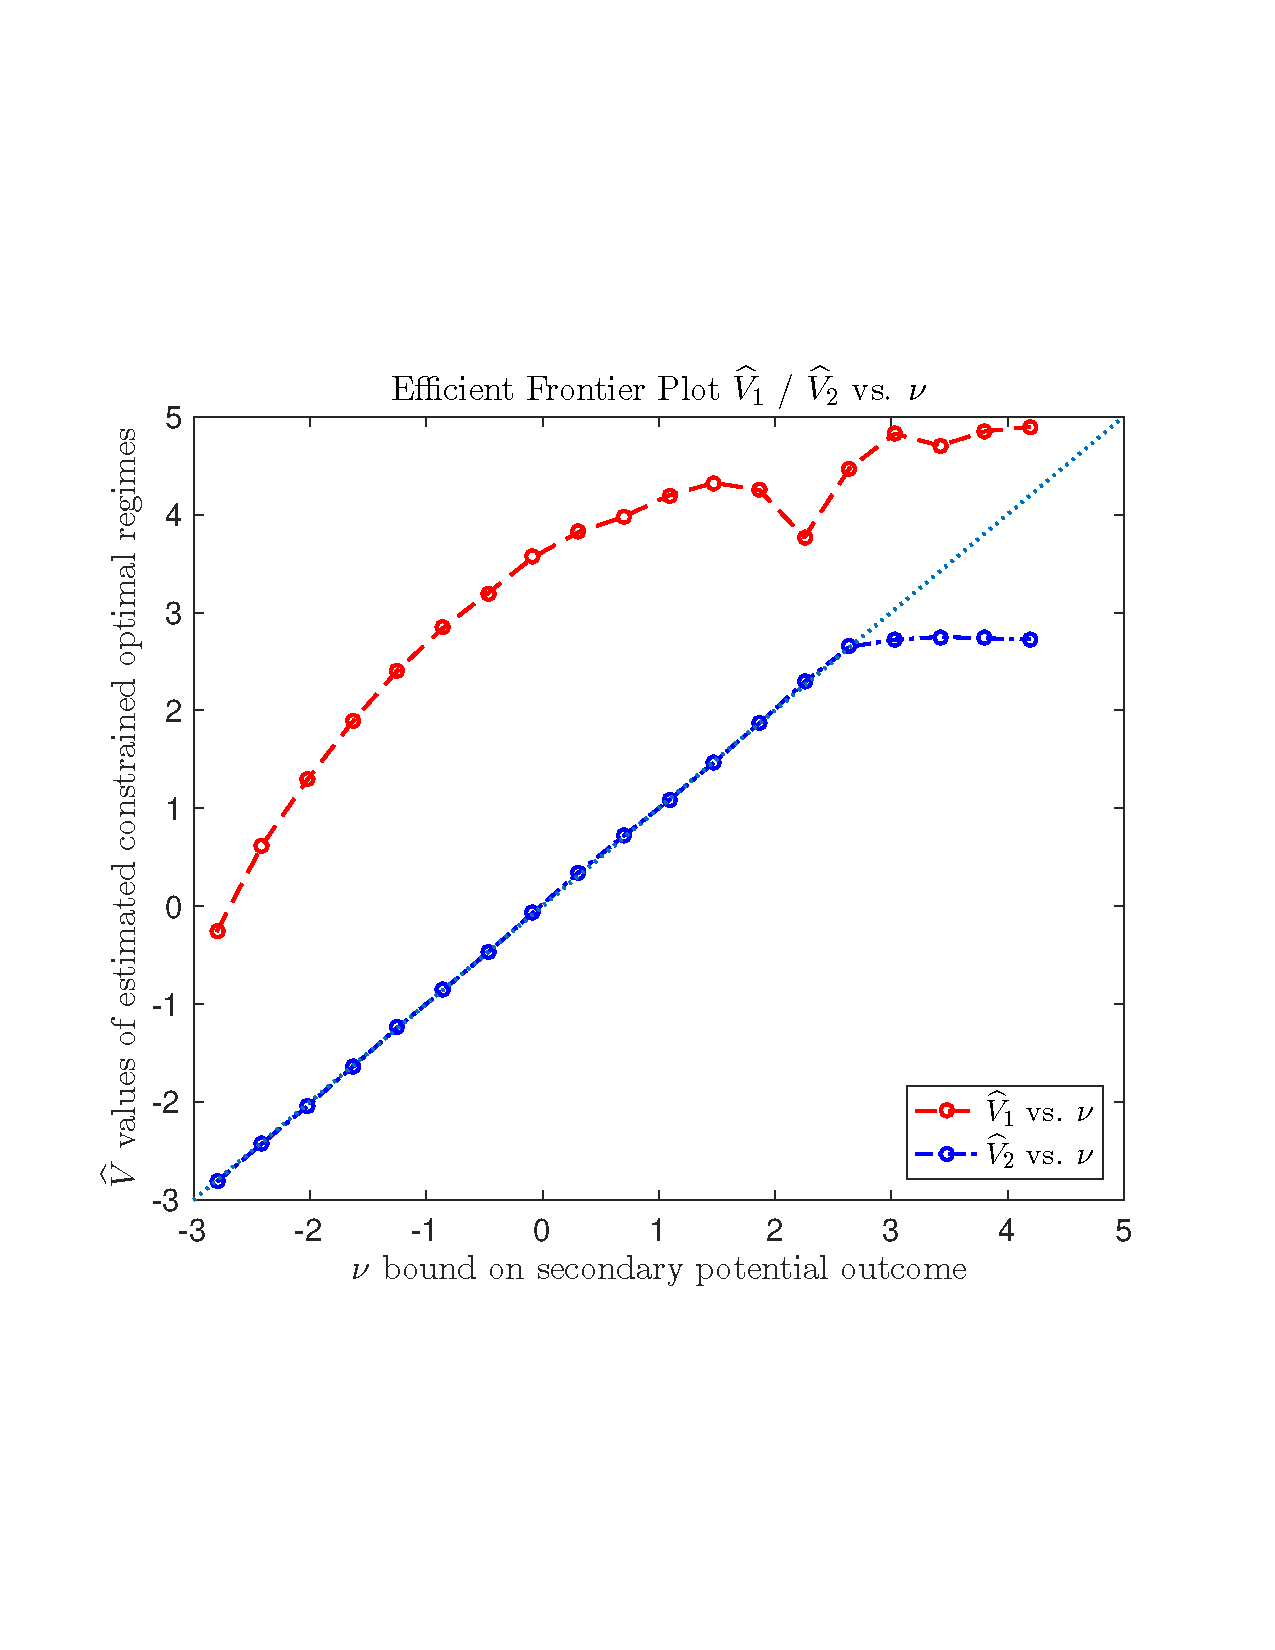
\includegraphics[width=\textwidth,height=\textheight,keepaspectratio]{//Users
/shuping.ruan/GitHub/thesis_research/Single-Stage-Constrained-Optimal
-Treatment-Regimes/plot_results/efficient_plot8.pdf}
%	\caption{Efficient frontier for estimated constrained optimal regimes
(single-stage) for Setting 8.}
%	\label{fig:8}
%\end{figure}	
%\end{frame}
%%%---
%\begin{frame}
%\begin{table}[!htbp]
% \resizebox{\textwidth}{!}{
%	\centering
%	{\tt
%	
\begin{tabular}{rrrrrrrrrr}\hline 
 $\nu$  & $\wh{V}_1(\wh{\bs{\theta}}_{\nu})$ & $std(\wh{V}_1)$ & $\wh{V}_2(\wh{\bs{\theta}}_{\nu})$ & $std(\wh{V}_2)$ & $\wh{\theta}_{\nu,1}$ & $std(\wh{\theta}_{\nu,1})$ & $\wh{\theta}_{\nu,2}$ & $std(\wh{\theta}_{\nu,2})$ \\ \hline 
-0.70 &     3.32 &     1.24  &    -0.97 &      0.63 &      0.75 &      0.04 &     -0.66 &      0.05 \\ 
-0.56 &     3.72 &     0.01  &    -0.77 &      0.02 &      0.73 &      0.04 &     -0.68 &      0.04 \\ 
-0.41 &     3.72 &     0.01  &    -0.77 &      0.02 &      0.73 &      0.04 &     -0.68 &      0.04 \\ 
-0.27 &     3.72 &     0.01  &    -0.77 &      0.02 &      0.73 &      0.04 &     -0.68 &      0.04 \\ 
-0.13 &     3.72 &     0.01  &    -0.77 &      0.02 &      0.73 &      0.04 &     -0.68 &      0.04 \\ 
 0.01 &     3.72 &     0.01  &    -0.77 &      0.02 &      0.73 &      0.04 &     -0.68 &      0.04 \\ 
 0.15 &     3.72 &     0.01  &    -0.77 &      0.02 &      0.73 &      0.04 &     -0.68 &      0.04 \\ 
 0.29 &     3.72 &     0.01  &    -0.77 &      0.02 &      0.73 &      0.04 &     -0.68 &      0.04 \\ 
 0.43 &     3.72 &     0.01  &    -0.77 &      0.02 &      0.73 &      0.04 &     -0.68 &      0.04 \\ 
 0.58 &     3.72 &     0.01  &    -0.77 &      0.02 &      0.73 &      0.04 &     -0.68 &      0.04 \\ 
 0.72 &     3.72 &     0.01  &    -0.77 &      0.02 &      0.73 &      0.04 &     -0.68 &      0.04 \\ 
 0.86 &     3.72 &     0.01  &    -0.77 &      0.02 &      0.73 &      0.04 &     -0.68 &      0.04 \\ 
 1.00 &     3.72 &     0.01  &    -0.77 &      0.02 &      0.73 &      0.04 &     -0.68 &      0.04 \\ 
 1.14 &     3.72 &     0.01  &    -0.77 &      0.02 &      0.73 &      0.04 &     -0.68 &      0.04 \\ 
 1.28 &     3.72 &     0.01  &    -0.77 &      0.02 &      0.73 &      0.04 &     -0.68 &      0.04 \\ 
 1.43 &     3.72 &     0.01  &    -0.77 &      0.02 &      0.73 &      0.04 &     -0.68 &      0.04 \\ 
 1.57 &     3.72 &     0.01  &    -0.77 &      0.02 &      0.73 &      0.04 &     -0.68 &      0.04 \\ 
 1.71 &     3.72 &     0.01  &    -0.77 &      0.02 &      0.73 &      0.04 &     -0.68 &      0.04 \\ 
 1.85 &     3.72 &     0.01  &    -0.77 &      0.02 &      0.73 &      0.04 &     -0.68 &      0.04 \\ \hline 
\end{tabular}

%	}}
%\caption {Simulation Result for Setting 9}
%\end{table} 	
%\end{frame}
%\begin{frame}
%\begin{figure}
%
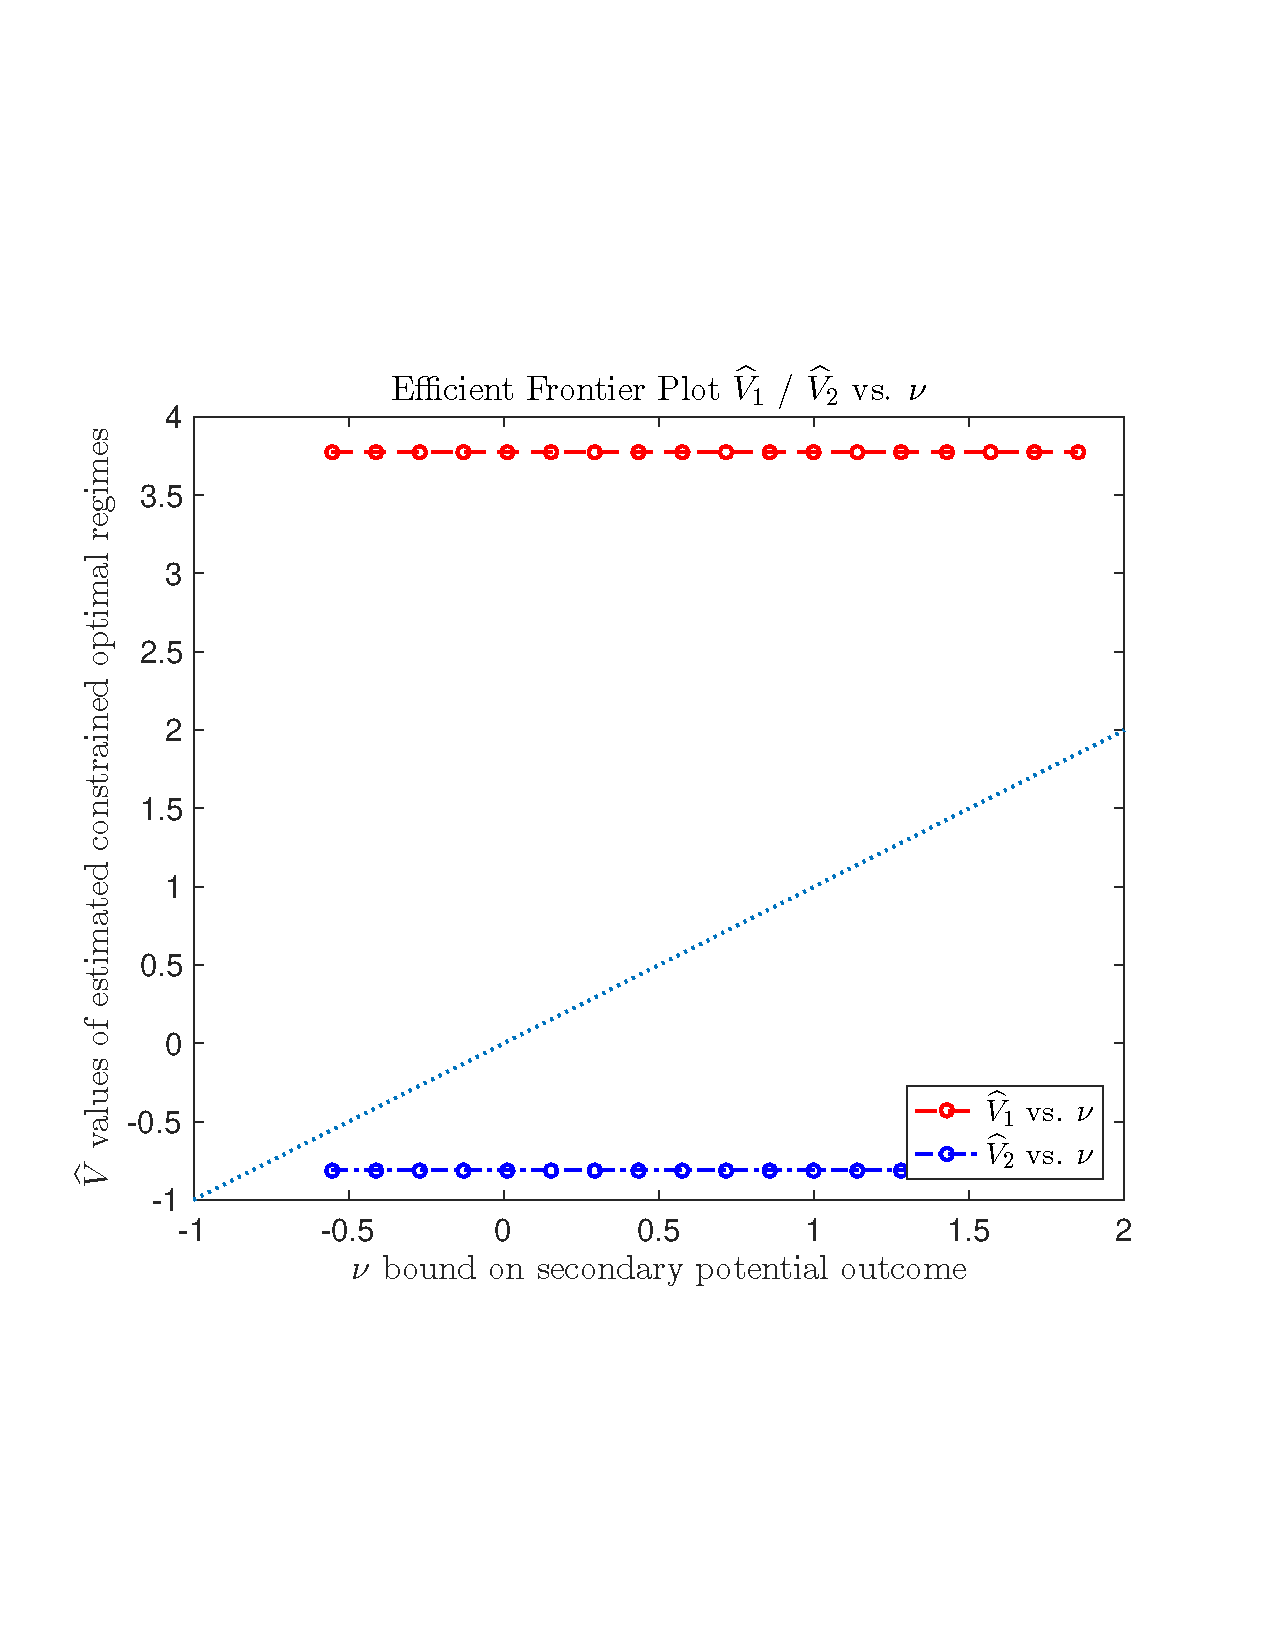
\includegraphics[width=\textwidth,height=\textheight,keepaspectratio]{//Users
/shuping.ruan/GitHub/thesis_research/Single-Stage-Constrained-Optimal
-Treatment-Regimes/plot_results/efficient_plot9.pdf}
%	\caption{Efficient frontier for estimated constrained optimal regimes
(single-stage) for Setting 9.}
%	\label{fig:9}
%\end{figure}	
%\end{frame}
%%%%%%%%%%%%%%%%%%%%%%%%%%%%%%%%%%%%%%%%%%%%%%%%%%%%%%%%%%%%%%%%%%%%%%
\section{Multi-stage}
\begin{frame}
  \frametitle{Data}
	\begin{itemize}
		\item  The dataset $$\{(\bs{X}_{1}^{i}, A_{1}^{i},\bs{X}_{2}^{i}, A_{2}^{i},
\cdots, \bs{X}_{T}^{i}, A_{T}^{i}, \bs{Y}^{i})\}_{i=1}^{n},$$
		\item $n$ i.i.d. patient trajectories
		%\item $\bs{X}_1$ be a patient baseline covariate
		\item $\bs{X}_t$, the patient covariate collected between the (t-1)-th
decision point and the t-th decision point
		\item $A_t$, the $t$th-stage treatment variable
		\item $\bs{Y}$, the final outcome vector. $Y_1$, the primary outcome of
interest, the higher the better; $Y_2, \cdots, Y_J$, the secondary outcomes of
interest, the lower the better. 
		\item Let $\bs{H}_t$ denote the patient history information up to the
decision point $t$, i.e., $\bs{H}^\itl_t = (\bs{H}^\itl_{t-1}, A_{t-1},
\bs{X}^\itl_t)$, $\cdots$
		\item $\br{A}_t = (A_1, A_2, \cdots, A_t)$ denotes a sequence of treatment
history up to time point $t$
	\end{itemize}
\end{frame}
\begin{frame}
	\frametitle{Potential outcome framework}
 \begin{itemize}
 	\item The set of potential outcomes is $\bs{W}^* = \{ \bs{X}^*_2(a_1),
\bs{X}^*_3(\br{a}_2), \cdots, \bs{X}^*_T(\br{a}_{T-1}), \bs{Y}^*_T(\br{a}_T),
\text{for all } \br{a}_t \in \br{\ml{A}}_t, t=1, 2, \cdots, T \}$% potential
outcome that would have been observed if the patient followed the treatment
history sequence $\br{a}_{t-1}$. 
 	\item Assumptions to connect  observed data w/ potential outcomes
 	\begin{itemize}
 		\item \textit{Consistency:}
 	 	$\bs{Y} = \bs{Y}^*(\br{A}_T)$, and $\bs{X}_t = \bs{X}^*_t(\br{A}_{t-1})$,
$t = 2, \cdots, T$.
 		\item \textit{Sequential randomization assumption:}
 		$A_{t}  \indep \bs{W}^*  \mid \bs{H}_{t}$, for $t =1 ,2, \cdots, T$.
 		\item \textit{Positivity assumption:} $\exists \, \epsilon_t > 0$, such that
$\text{Pr}(A_t = a_t \mid \bs{H}_t) > \epsilon_t$, w/ prob 1, for all $a_t \in
\ml{A}_t$, $t=1, 2, \cdots, T$.
 	\end{itemize}
 \end{itemize}
 \end{frame}
 \begin{frame}
 \frametitle{Values of a regime}
 \begin{itemize}
 \item The values of a dynamic treatment regime, $\bs{V}(\bs{\pi}) =
\mb{E}\bs{Y}^*(\bs{\pi})$, is defined as the expected final outcome if each
patient in the population of interest is treated according to $\bs{\pi}$. 
 \item Values of a regime are estimated using G-computation and the
mean-variance modeling techniques by Linn et al.
 %\item The Q functions 	
 %		$$Q(H_1, A_1) = \mb{E}(Q^{\pi}(H_1, \pi))$$
 \end{itemize}
\end{frame}
%\begin{frame}
%\frametitle{Potential outcome framework}
%\begin{itemize}
%%\item This assumptions imply that 
%%\begin{itemize}
%%\item $\txt{Pr}(\bs{Y}^*(\br{a}_T) \le \bs{y} \,| \, \bs{H}^*_T(\br{a}_{T-1})
=\bs{h}_T) = \txt{Pr}(\bs{Y} \le \bs{y} \, |\,  \bs{H}_T = \bs{h}_T, A_T=a_T)$

%%\item $\txt{Pr}(\bs{X}_{t+1}^*(\br{a}_{t}) \le \bs{x}_{t+1} \,|\,
\bs{H}^*_t(\br{a}_{t-1}) = \bs{h}^*_t) = \txt{Pr}(\bs{X}_{t+1} \le \bs{x}_{t+1}
\mid  \bs{H}_t = \bs{h}_t, A_t=a_t)$ for $t = 1, 2, \cdots, T-1$. 
%%\end{itemize}
%
%\item Hence, we can estimate the values of a regime using the observed dataset
using G-computation formula, and the mean-variance modeling techniques by Linn
et al.
%%\begin{eqnarray*}
%%&& \text{Pr}\lt( Y_j^*({\bs{\pi}}) \le y_j  \rt)  = F_{Y_j^*({\bs{\pi}})}\lt(
y_j  \rt) \\
%%&& = \idotsint F_{Y_j\rvert \bs{H}_T, A_T}\lt(y_j \rvert \bs{h}_T,
\pi_T(\bs{h}_T) \rt) \\
%%&& \,d F_{\bs{H}_T \rvert \bs{H}_{T-1}, A_{T-1}}\lt( \bs{h}_T \rvert
\bs{h}_{T-1}, \pi_{T-1}(\bs{h}_{T-1}) \rt) \\ 
%%&& \,d F_{\bs{H}_{T-1} \rvert \bs{H}_{T-2}, A_{T-2}}\lt( \bs{h}_{T-1} \rvert
\bs{h}_{T-2}, \pi_{T-2}(\bs{h}_{T-2}) \rt)
%%\cdots\\
%%&& \,d F_{\bs{H}_2\rvert \bs{H}_{1}, A_{1}}\lt( \bs{h}_2 \rvert \bs{h}_{1},
\pi_{1}(\bs{h}_{1}) \rt)\,d F_{\bs{H}_1}(\bs{h}_1)
%%\end{eqnarray*}
%\end{itemize}
%\end{frame}
%\begin{frame}
%\frametitle{Potential outcome framework}
%\begin{itemize}
%\item A dynamic treatment regime, $\bs{\pi} = (\pi_1, \pi_2, \cdots, \pi_T)$,
is a sequence of decision rules. 
%\item Each decision rule, $\pi_t : \text{supp}( \bs{H}_t ) \to \ml{A}_t$, is a
function that maps the support of patient history information $\bs{H}_t$ to the
set of all possible treatments at time point $t$. 
%\item The final potential outcome under the regime $\bs{\pi}$ is
$\bs{Y}^*(\bs{\pi}) = \sum_{\br{a}_T \in
\br{\ml{A}}_T}\bs{Y}^*(\br{a}_T)\mb{I}(\bs{\pi} = \br{a}_T)$
%\item The intermediate potential outcome under that regime is
$\bs{X}_{t+1}^*(\bs{\pi}_{t}) = \sum_{\br{a}_t \in
\br{\ml{A}}_t}\bs{X}_{t+1}^*(\br{a}_{t})\mb{I}(\bs{\pi}_t = \br{a}_t)$, where
$\bs{\pi}_t = (\pi_1, \pi_2, \cdots, \pi_t)$.	
%\item The value of a dynamic treatment regime, $\bs{V}(\bs{\pi}) =
\mb{E}\bs{Y}^*(\bs{\pi})$, is defined as the expected final outcome if each
patient in the population of interest is treated according to $\bs{\pi}$. Each
component of $\bs{V}(\bs{\pi})$ is denoted by $V_j(\bs{\pi}) =
\mb{E}Y_j^*(\bs{\pi})$, for $j = 1, \cdots, J$.	
%\end{itemize}
%\end{frame}
%\begin{frame}
%\begin{itemize}
%\item The value of a dynamic treatment regime, $\bs{V}(\bs{\pi}) =
\mb{E}\bs{Y}^*(\bs{\pi})$, is defined as the expected final outcome if each
patient in the population of interest is treated according to $\bs{\pi}$. Each
component of $\bs{V}(\bs{\pi})$ is denoted by $V_j(\bs{\pi}) =
\mb{E}Y_j^*(\bs{\pi})$, for $j = 1, \cdots, J$.	
%\end{itemize}
%\end{frame}
\begin{frame}
\frametitle{Constrained optimal treatment regimes}
\begin{itemize}
%\item  Our goal is to find a constrained optimal regime,
$\bs{\pi}_{\bs{\nu}}^{*}$, which maximizes the expectation of the primary final
potential outcome $V_1\left( \bs{\pi}\right) $, subject to an upper bound
constraints on the expectation of the secondary final potential outcomes
$V_j\left( \bs{\pi}\right)$, for $j=2 ,\cdots, J$.
\item A multi-stage constrained optimal treatment regime
\begin{equation*}
\begin{gathered}
 \underset{\bs{\pi} \in \bs{\Pi}}{\txt{max}} \,\,
 V_1( \bs{\pi} )  \\
  \txt{subject to}  \,\, V_j( \bs{\pi} ) \le \nu_{j-1},
\end{gathered}
\end{equation*}
where $j = 2, 3, \cdots, J$  and $\bs{\Pi}$ is the class of dynamic treatment
regimes under consideration. %The feasible space of the class of regimes,
$\ml{F}(\bs{\Pi})$, is the set of all regimes satisfying the constraints. % For
each $\bs{\pi} \in \ml{F}(\bs{\Pi})$, $V_j(\bs{\pi}) \le \nu_{j-1}$, for $j =
2, \cdots, J$. Then, a multi-stage constrained optimal regime can also be
written as $\bs{\pi}_{\bs{\nu}}^*= \text{argmax}_{{\bs{\pi} \in
\ml{F}(\bs{\Pi})}}V_1 (\bs{\pi})$.	
\end{itemize}
\end{frame}
\begin{frame}
	\frametitle{Constrained optimal treatment regimes}
\begin{itemize}
\item Linear decision rules for each stage, $\pi_t(\bs{h}_t) =
\tsgn(\bs{h}^{\itl}_t\bs{\theta}_t)$, and
$\bs{\theta}^{\itl}_t\bs{\theta}_t=1$.
\item Interior-point method 
\begin{flalign*}
\min_{\bs{\theta}, \bs{z}} {\phi}_{\mu}(\bs{\theta}, \bs{z}) =
{v}_1(\bs{\theta}) - \mu \sum_{j=2}^J \ln z_j,\\
\text{subject to }{v}_j(\bs{\theta}) +z_j = 0, h_t(\bs{\theta}_t) = 0,
\end{flalign*}
where ${v}_1(\bs{\theta}) = -{V}_1(\bs{\theta})$,
${v}_j(\bs{\theta})={\bs{V}}_j(\bs{\theta}) -\nu_j$ for $j = 2, \cdots, J$, and
$h_t(\bs{\theta}_t) = \bs{\theta}_t^{\itl}\bs{\theta}_t - 1$ for $t = 1,
\cdots, T$. 
%\item Penalty-barrier method
%\begin{equation*}
%\min_{\bs{\theta}} \wh{\phi}^{BP}_{\mu}(\bs{\theta}) = \min
\wh{v}_1(\bs{\theta}) - \mu \sum_{j=2}^J \ln \wh{v}_j(\bs{\theta}) +
\frac{1}{2\mu}\sum_{t=1}^{T}(\bs{\theta}^{\itl}_t\bs{\theta}_t - 1)^2.
%\end{equation*}
\end{itemize}
\end{frame}
%\begin{frame}
%\frametitle{Estimation of the values of a regime}
%To estimate the values of a regime, we use the G-computation formula by
Robins, etc~\cite{Gill2001}. For any arbitrary regime $\bs{\pi} = (\pi_1,
\cdots, \pi_T) $, assume the three causal assumptions are satisfied, then for
each component of $\bs{Y}$
%\end{frame}
\begin{frame}
\frametitle{Simulation design}
%We demonstrate our proposed method using the toy example presented by Linn et
al~\cite{constrained}, where there are two competing outcomes $Y$ and $Z$. The
goal is to maximize the mean of $Y$, subject to an upper bound on the mean of
$Z$. $Y$ is coded so that the higher the value the better, such as the
effectiveness of the treatment regimes. Meanwhile, $Z$ is coded the lower the
better, such as the side-effect burden. The model for generating the patient
trajectories $(X_1, A_1, X_2, A_2, Y, Z)$ are as follow:
This model is a simple representation of the data from a two-stage sequential
randomized trials. 
\begin{flalign*}
&X_1 \sim \text{Normal}(1,1), \bs{H}_1 = (1, X_1)^{\itl}, \\
&A_1 \sim \text{Uniform}\left\{-1, 1\right\}, \\
&X_2 = \bs{H}_1^{\itl}\bs{\beta}_{1,0} + A_1\bs{H}_1^{\itl}\bs{\beta}_{1,1} +
\epsilon, \epsilon \sim \text{Normal}(0,1), \\
&\bs{H}_2 = (1, X_2)^{\itl},\\
&A_2 \sim \text{Uniform}\left\{-1, 1\right\}, \\
&Y = \bs{H}_2^{\itl}\bs{\beta}_{2,0,Y} + A_2
\bs{H}_2^{\itl}\bs{\beta}_{2,1,Y}+\epsilon_Y \\
&Z = \bs{H}_2^{\itl}\bs{\beta}_{2,0,Z} + A_2
\bs{H}_2^{\itl}\bs{\beta}_{2,1,Z}+\epsilon_Z \\
&(\epsilon_Y, \epsilon_Z)^{\itl} \sim \text{Normal}(\bs{0}_2, \Sigma_{Y,Z}) 
\end{flalign*}
%Variable $X_1$ represents the summary of patient status before the first
treatment assignment $A_1$. Variable $X_2$ represents the summary of patient
status before the second treatment assignment $A_2$. The parameters involved
are set to the following,
%\begin{flalign*}
%&\bs{\beta}_{1,0} = (0.5, 0.75)^{\itl}\\
%&\bs{\beta}_{1,1} = (0.25, 0.5)^{\itl}\\
%&\bs{\gamma}_0 = (0.25, -0.05)^{\itl}\\
%&\bs{\gamma}_1 = (0.1, -0.05)^{\itl}\\
%&\bs{\beta}_{2,0,Y} = (30, 2)^{\itl}\\
%&\bs{\beta}_{2,1,Y} = (5, -1.5)^{\itl}\\
%&\bs{\beta}_{2,0,Z} = (15, 1)^{\itl}\\
%&\bs{\beta}_{2,1,Z}=(3,-0.5)^{\itl}\\
%&\Sigma_{Y,Z} = \begin{bmatrix}
%1.0, &0.7 \\
%0.7,& 1.0
%\end{bmatrix}
%\end{flalign*}
The class of regimes under consideration is $\pi_1 =
\text{sgn}(\bs{h}_1^{\itl}\bs{\theta}_1)$ and  $\pi_2 =
\text{sgn}(\bs{h}_2^{\itl}\bs{\theta}_2)$.% where $\bs{\theta}_1$ and
$\bs{\theta}_2$ are the index parameters for the regimes. %The true optimal
regimes are denoted by $d^{*}_1 = \text{sgn}(\bs{h}_1^{\itl}\bs{\theta}^{*}_1)$
and  $d^{*}_2 = \text{sgn}(\bs{h}_2^{\itl}\bs{\theta}^{*}_2)$. The estimated
optimal regimes are denoted by $\wh{d}_1 =
\text{sgn}(\bs{h}_1^{\itl}\wh{\bs{\theta}}_1)$ and  $\wh{d}_2 =
\text{sgn}(\bs{h}_2^{\itl}\wh{\bs{\theta}}_2)$. Here, the sgn function is
defined as
% \begin{gather*}
%\text{sgn}(x)=\begin{cases}
%1 & \mbox{if }x\ge0,\\
%-1 & \mbox{if }x<0.
%\end{cases}
%\end{gather*}	
\end{frame}
%\begin{frame}
%\frametitle{Simulation results}
%%We summarize the simulation results here. Figure 2. below shows the estimated
optimal regime values and their standard deviation. Figure 2.1 is the efficient
frontier plot. The red dashed line represents $\wh{V}_1$ under estimated
constrained optimal regime, and the blue dash-dotted line represents $\wh{V}_2$
under that regime. The plot represents the best possible value of the primary
potential outcome for its level of risk, which is the value of the secondary
potential outcome. In the plot, the value of the primary outcome increases as
the constraint bound gets looser. Meanwhile the value of the secondary outcome
keep up with the constraint, until the constraint is not effective. Once the
constraint gets larger than the maximum value of the secondary potential
outcome, the constrained problem becomes an unconstrained problem. \\
%%\begin{table}[tp]
%%\centering
%%{\tt
%%
\begin{tabular}{rrrrr}\hline 
$\nu$  & $\wh{V}_1(\wh{\bs{\theta}}_{\nu})$ & $std(\wh{V}_1)$ & $\wh{V}_2(\wh{\bs{\theta}}_{\nu})$ & $std(\wh{V}_2)$ \\ \hline 
   12.86 &    27.48 &     0.46  &    12.86 &      0.23  \\ 
   13.45 &    28.90 &     0.42  &    13.37 &      0.15  \\ 
   14.03 &    30.38 &     0.64  &    13.89 &      0.17  \\ 
   14.62 &    31.85 &     0.83  &    14.46 &      0.16  \\ 
   15.21 &    33.53 &     0.64  &    15.05 &      0.13  \\ 
   15.79 &    34.47 &     0.70  &    15.64 &      0.14  \\ 
   16.38 &    35.47 &     0.94  &    16.15 &      0.29  \\ 
   16.97 &    36.33 &     0.93  &    16.68 &      0.40  \\ 
   17.55 &    37.08 &     0.87  &    17.31 &      0.41  \\ 
   18.14 &    37.62 &     0.51  &    17.89 &      0.31  \\ 
   18.72 &    37.79 &     0.72  &    18.32 &      0.44  \\ 
   19.31 &    38.03 &     0.17  &    18.91 &      0.10  \\ 
   19.90 &    38.03 &     0.17  &    18.91 &      0.10  \\ 
   20.48 &    38.03 &     0.17  &    18.91 &      0.10  \\ 
   21.07 &    38.03 &     0.17  &    18.91 &      0.10  \\ 
   21.66 &    38.03 &     0.17  &    18.91 &      0.10  \\ 
   22.24 &    38.03 &     0.17  &    18.91 &      0.10  \\ 
   22.83 &    38.03 &     0.17  &    18.91 &      0.10  \\ 
   23.41 &    38.03 &     0.17  &    18.91 &      0.10  \\ 
   24.00 &    38.03 &     0.17  &    18.91 &      0.10  \\ \hline 
\end{tabular}
%%}
%%%\caption{Simulation results}
%%\end{table}
%\begin{minipage}{0.2\textwidth}
%\centering
%\begin{table}
%\begin{tabular}{rrrrr}\hline 
%$\nu$  & $\wh{V}_1(\wh{\bs{\theta}}_{\nu})$ & $std(\wh{V}_1)$ &
$\wh{V}_2(\wh{\bs{\theta}}_{\nu})$ & $std(\wh{V}_2)$ \\ \hline 
%   12.86 &    27.48 &     0.46  &    12.86 &      0.23  \\ 
%   13.45 &    28.90 &     0.42  &    13.37 &      0.15  \\ 
%   14.03 &    30.38 &     0.64  &    13.89 &      0.17  \\ 
%   14.62 &    31.85 &     0.83  &    14.46 &      0.16  \\ 
%   15.21 &    33.53 &     0.64  &    15.05 &      0.13  \\ 
%   15.79 &    34.47 &     0.70  &    15.64 &      0.14  \\ 
%   16.38 &    35.47 &     0.94  &    16.15 &      0.29  \\ 
%   16.97 &    36.33 &     0.93  &    16.68 &      0.40  \\ 
%   17.55 &    37.08 &     0.87  &    17.31 &      0.41  \\ 
%   18.14 &    37.62 &     0.51  &    17.89 &      0.31  \\ 
%   18.72 &    37.79 &     0.72  &    18.32 &      0.44  \\ 
%   19.31 &    38.03 &     0.17  &    18.91 &      0.10  \\ 
%   19.90 &    38.03 &     0.17  &    18.91 &      0.10  \\ 
%   20.48 &    38.03 &     0.17  &    18.91 &      0.10  \\ \hline 
% %  21.07 &    38.03 &     0.17  &    18.91 &      0.10  \\ 
% %  21.66 &    38.03 &     0.17  &    18.91 &      0.10  \\ 
% %  22.24 &    38.03 &     0.17  &    18.91 &      0.10  \\ 
% %  22.83 &    38.03 &     0.17  &    18.91 &      0.10  \\ 
% %  23.41 &    38.03 &     0.17  &    18.91 &      0.10  \\ 
% %  24.00 &    38.03 &     0.17  &    18.91 &      0.10  \\ \hline 
%\end{tabular}	
%\end{table}
%\end{minipage}
%\end{frame}
\begin{frame}
\begin{figure}[H]
	\centering
	\includegraphics[width=\textwidth,height=\textheight,keepaspectratio]{/Users
/shuping.ruan/Dropbox/Apps/Texpad/Graduate/thesis/Chapter-2/figs/efficient
_plot.pdf}
	\caption{Efficient frontier for estimated constrained optimal regimes
(multi-stage)}
\end{figure}	
\end{frame}



 %%%%%%%%%%%%%%%%%%%%%%%%%%%%%%%%%%%%%%%%%%%%%%%%%%%%%%%%%%%%%%%%%%%%%%
\section{Infinite-stage}
\begin{frame}
\frametitle{Constrained reinforcement learning}
\begin{itemize}
\item Patients with chronic diseases are often monitored and treated throughout
their life. 
\begin{itemize}
	\item Real-time actions 
	\item No a-priori fixed end point 
	\item Infinite stage reinforcement learning 
\end{itemize}
\item Adopt the constrained Markov Decision Processes (cMDPs) framework for
infinite horizon. %CMDPs are a well-studied framework for reinforcement
learning under constraints. 
%\item The goal is to find the optimal policy, while satisfying constraints on
expectations of secondary costs. For many applications of reinforcement
learning, the constrained approach is more intuitive and more practical than
eliciting a single reward function in order to achieve desirable results. For
instance, satisfying safety constraints is necessary for systems that
physically interact with humans. 
\item Previously, linear programming is used to sought out constrained optimal
policies in the setting of finite cMDPs with known models. 
\item However, few methods have been proposed for high-dimensional constrained
reinforcement learning problems w/o modeling the underlying dynamics.
%Recently, Achiam et al~\cite{Achiam2017} proposed constrained policy
optimization, a general-purpose policy search algorithm for constrained
reinforcement learning guaranteeing near-constraint satisfaction at each
iteration. Taking into the consideration of properties of clinical application,
such as data scarcity and off-policy learning, we develop an algorithm by
taking advantage of least-squares policy evaluation and interior-point method
for estimating constrained optimal dynamic treatment regimes. Our method is
applied to a simulated cancer trial dataset based on a chemotherapy
mathematical model.	
\end{itemize}
\end{frame}
\begin{frame}
 \frametitle{Data}
  \begin{itemize}
  %\item We use dataset observed over a finite length of time steps to
construct a regime in the setting of infinite horizon Markov decision process.

  \item The structure of the available data is  $\bs{D} = \lt\{  (\bs{S}^i_{0},
A^i_{0}, \bs{R}^i_{0} , \bs{S}^i_{1}, \cdots, 
 \bs{S}^i_{T_i-1} , A^i_{T_i-1}, \bs{R}^i_{T_i-1}, \bs{S}^i_{T_i})
\rt\}_{i=1}^n,$
 \item $n$ i.i.d. patient trajectories.
  \item For each patient, his/er follow up time length $T_i$ may be different. 
  \item $\bs{S}_{t} \in \bs{\ml{S}}$ denotes a vector of patient clinical
information recorded up to and including time point $t$ %referred as
\textit{state} in the reinforcement learning (RL) vocabulary.
  \item $A_{t} \in \ml{A}$ denotes the treatment assignment at time point $t$
after measuring $\bs{S}_{t},$ % referred as \textit{action} in RL. 
  \item  $\bs{R}_{t} \in \mb{R}^J$ is the reward obtained after treatment
$A_{t}$ is assigned. %We assume the reward, possibly defined based on domain
expertise, is known vector-valued function $\bs{r}$: $\bs{\ml{S}} \times \ml{A}
\times \bs{\ml{S}} \to \mb{R}^J $, so that $\bs{R}_{t} = \bs{r}(\bs{S}_{t},
A_t,
\bs{S}_{t+1})$. The vector-valued reward function is the same across all the
time points $t$ as well.
  %\item  Moreover, if a patient dies during the follow-up, say at decision
point $t$, we set $\bs{S}_t = \bs{\emptyset}$, referred as the absorbing state
in RL. Then, the patient's treatment assignment at time $t$ is $A_t=\emptyset$,
and his/er length of follow-up $T = t$.	
    \end{itemize}
\end{frame}
\begin{frame}
\frametitle{Potential outcome frameworks}
\begin{itemize}
\item Let $\br{\bs{a}}_{t} = (a_0, a_1, \cdots, a_t) \in \br{\bs{\ml{A}}}_{t}$
be a possible treatment assignment sequence up to time point $t$.
\item Let $\br{\bs{s}}_{t} = (\bs{s}_0, \bs{s}_1, \cdots, \bs{s}_t) \in
\br{\bs{\ml{S}}}_{t}$ be a possible state sequences up to time point $t$, $t
\ge 0$.
\item The set of potential outcomes is $\bs{W}^* = \lt\{\bs{S}^*_1(a_0),
\bs{S}^*_2(\br{\bs{a}}_1),\cdots,  \bs{S}^*_{t+1}(\br{\bs{a}}_{t}), \cdots,
\text{ for all } \br{\bs{a}}_{\infty} \in \br{\bs{\ml{A}}}_{\infty} \rt\}$,
where $\bs{S}^*_{t+1}(\br{\bs{a}}_{t})$ is the potential state at $(t+1)$-th
time point that would have been observed if the individual had been assigned
the treatment sequence $\br{\bs{a}}_{t}$, $t \ge 0$.
\end{itemize}
 %Moreover, if $\bs{S}_{t+1}^*(\br{\bs{a}}_{t}) = \bs{\emptyset}$ happens at
time point $t+1$, then $\bs{S}_{t+2}^*(\br{\bs{a}}_{t+1})
=\bs{S}_{t+3}^*(\br{\bs{a}}_{t+2}) = \cdots = \bs{\emptyset}$, which indicates
the patient, if followed treatment assignment sequence $\br{\bs{a}}_t$, would
have died at time point $t+1$ in the counter-factual world.  Rewards with
respect to potential states are $\bs{R}^*_t = \bs{r}(\bs{S}^*_t, A_t,
\bs{S}^*_{t+1})$. The following assumptions are made in the potential outcome
framework	
\end{frame}
\begin{frame}
\frametitle{Potential outcome frameworks}
	\begin{itemize}
	\item \textit{Consistency}:  $\bs{S}_{t+1} = \bs{S}^*_{t+1}(\br{\bs{A}}_{t})$,
for all $t \ge 0$.
	\item \textit{Sequential randomization assumption}: $A_{t+1} \indep \bs{W}^*
\mid \br{\bs{S}}_{t+1}, \br{\bs{A}}_{t},$ for all $t \ge 0$.
	\item \textit{Positivity}: there exists $\epsilon_0 > 0$, so that $P\lt(
A_{t+1} = a_{t+1} \mid \br{\bs{S}}_{t+1} = \br{\bs{s}}_{t+1}, \br{\bs{A}}_{t} =
\br{\bs{a}}_{t} \rt) > \epsilon_0$, for all $a_{t+1} \in \mathcal{A}$,
$\br{\bs{a}}_{t} \in \br{\bs{\ml{A}}}_t$ and $\br{\bs{s}}_{t+1} \in
\br{\bs{\ml{S}}}_{t+1}$, and all $t \ge 0$.
	\end{itemize}
% These assumptions link the potential outcome and the observed data, and are
guaranteed in well-designed Sequential, Multiple Assignment, Randomized Trials
(SMARTs).  Therefore, the observed data from those trials are used to infer the
average causal effect of a regime of interest.  	 
\end{frame}
\begin{frame}
\frametitle{Markov Decision Process}
\begin{itemize}       
\item \textit{Markov assumption}: $\bs{S}_{t+1} \indep \lt( \br{\bs{A}}_{t-1},
\br{\bs{S}}_{t-1} \rt) \mid \lt( A_{t}, \bs{S}_{t} \rt) $, for all $t \ge 1$.
\item \textit{Time homogeneity}: the conditional density	$P_t(\bs{S}_{t+1} =
\bs{s}^{\prime} \mid A_{t} = a, \bs{S}_{t} = \bs{s} ) = P(\bs{s}^{\prime} \mid
a, \bs{s})$ for all $\bs{s} , \bs{s}^{\prime} \in \bs{\mathcal{S}}$ and $a \in
\mathcal{A}$ and $t \ge 0$, where $\bs{s}$ and $\bs{s}^{\prime}$ denote the
current state and the next state, respectively. 
\end{itemize}
\end{frame}
\begin{frame}
\frametitle{Value functions of dynamic treatment regimes}
\begin{itemize}
\item A dynamic treatment regime, $\pi : \bs{\ml{S}} \to \mathcal{A}$.%., is
defined as a function which maps the support of the state variable to the set
of the possible treatment assignments. 
%\item As time homogeneity is assumed, we consider only stationary
deterministic regimes, where this mapping function $\pi(\bs{s})$ does not
change over time. Hence, a patient with state $\bs{S}_t = \bs{s}$ at time point
$t$ will be assigned with treatment $A_t = \pi\lt(\bs{s}\rt)$ for all $t$.  
\item The value function $\bs{V}^{\pi}\lt(\bs{s}\rt)$ of a state under a
certain policy $\pi$ is defined as the expected total discounted rewards when
the process begins in state $\bs{s}$ and all decisions are made according to
policy $\pi$. 
\item $\bs{V}^{\pi}\lt(\bs{s}\rt) = \mb{E}_{\bs{s}}^{\pi} \sum_{t=0}^{\infty}
\gamma^{t} \, \bs{r}(\bs{s}_t, a_t, \bs{s}_{t+1})$.%, where
$\mb{E}_{\bs{s}}^{\pi}$ is the expectation when the initial state is $\bs{s}$
and a policy $\pi$ is followed. 
\item Bellman equation, $\bs{V}^{\pi}\lt(\bs{s}\rt) =
\sum_{\bs{s}^{\prime}\in\bs{\ml{S}}}  p(\bs{s}^{\prime} \mid \bs{s},
\pi(\bs{s})) \lt(\bs{R}(\bs{s}, \pi(\bs{s}), \bs{s}^{\prime}) + \gamma
\bs{V}^{\pi}(\bs{s}^{\prime})\rt)$. % Here, $\bs{V}^{\pi}(\bs{s}) \in \mb{R}^J$
has the same dimensionality as the reward vector $\bs{R}$, as we are
considering multiple reward functions instead of a scalar reward function.

\end{itemize}
\end{frame}
\begin{frame}
\begin{itemize}
\frametitle{Value functions of dynamic treatment regimes}
\item Moreover, the state-action value function under policy $\pi$,
$\bs{Q}^{\pi}(\bs{s}, a) =\sum_{\bs{s}^{\prime} \in \bs{\ml{S}}} 
p\lt(\bs{s}^{\prime} \mid \bs{s}, a\rt) \lt( \bs{R}\lt(\bs{s}, a,
\bs{s}^{\prime}\rt) + \gamma \, \bs{Q}^{\pi}(\bs{s}^{\prime},
\pi(\bs{s}^{\prime}) ) \rt)$,
is defined similar but the first step takes action $a$. % and
$\bs{Q}^{\pi}(\bs{s}, a) \in \mb{R}^J$.
\item In clinical cases, the transition model $\mb{P}$ is unknown, optimal
regimes must be learn from observed dataset. 
\item In infinite horizon setting, as time steps are dropped, we break $n$
observed trajectories into 4-tuple of $(\bs{s}, a, \bs{r}, \bs{s}^{\prime})$
for estimating value functions. % The counter-factual assumptions
\textit{(A1-A3)} rule out the confounding phenomena and guarantee the
identifiability of the average causal effect of a regime	
\end{itemize}
\end{frame}
\begin{frame}
\frametitle{Least-squares policy evaluation}
\begin{itemize}
\item The state-action value function $\bs{Q}^{\pi}$ is considered the fixed
point of the Bellman operator: $\bs{Q}^{\pi}=T^{\pi}\bs{Q}^{\pi}$, where the
Bellman operator defined as  $$T^{\pi}\bs{Q}^{\pi} =\sum_{\bs{s}^{\prime} \in
\ml{S}}  p(\bs{s}^{\prime} | \bs{s}, a) \lt( \bs{R}(\bs{s}, a, \bs{s}^{\prime})
+ \gamma \sum_{a^{\p} \in \ml{A}} \pi(a^{\prime} \mid \bs{s}^{\p} )
\,\bs{Q}^{\pi}(\bs{s}^{\prime}, a^{\prime}) \rt).$$	
% \item %As $\bs{Q}(\bs{s},a) = (Q_1(\bs{s},a), Q_2(\bs{s},a), \cdots,
Q_{J}(\bs{s},a))^{\intercal}$,
\item  The approximation for each component is $Q_j^{\pi}(\bs{s},a;w) =
\sum_{k=1}^K \phi_{j,k}(\bs{s},a)w_{j,k} =  \bs{\phi}_{j}^{\intercal}(\bs{s},
a)\bs{w}_j$
\begin{itemize}
\item $\bs{w}_j = (w_{j,1}, \cdots, w_{j,K})^{\intercal}$ are the parameters to
estimate. 
\item The basis functions $\bs{\phi}_{j}(\bs{s}, a) = (\phi_{j,1}(\bs{s}, a),
\cdots, \phi_{j,K}(\bs{s}, a))^{\intercal}$ are arbitrary and fixed, which are
often non-linear functions of $\bs{s}$ and $a$.
\end{itemize}
% Moreover, % It is also required that the basis functions $\phi_{j,k}$ are
linearly independent to ensure that there are no redundant parameters and that
the matrices involved in the computations are full rank.
\end{itemize}
\end{frame}
\begin{frame}
\frametitle{Least-squares policy evaluation}
\begin{algorithm}[H]
	\caption{Least-squares policy evaluation LSQ}
	 \SetKwInOut{Input}{Input}
	\SetKwInOut{Output}{Output}
	\Input{A sample set $\bs{D}$ of 4 tuples $(\bs{s}^{\prime}, a, \bs{s},
\bs{r})$ \\
	$k$: Number of basis functions \\
	$\phi$: Basis functions \\
	$\gamma$: Discount factor \\
	$\pi$: policy whose value function is sought}
	\Output{Weights $\wh{\bs{w}}^{\pi}$}
	\BlankLine
	\BlankLine
	$\wh{\bs{A}} \leftarrow 0$ \hspace{25pt} // $(k\times k)$ matrix\\
	$\wh{\bs{b}} \leftarrow 0$ \hspace{28pt} // $(k\times 1)$ vector\\
	for each $(\bs{s}, a, \bs{r}, \bs{s}^{\prime}) \in \bs{D}$\\
	\hspace{25pt} $\wh{\bs{A}} \leftarrow \wh{\bs{A}} + \phi(\bs{s},
a)\lt(\phi(\bs{s}, a) - \gamma\phi(\bs{s}^{\prime},
\pi(\bs{s}^{\prime}))\rt)^{\intercal}$ \\
	\hspace{25pt} $\wh{\bs{b}} \leftarrow
	\wh{\bs{b}} + \phi(\bs{s}, a)\bs{r}$\\
	$\wh{\bs{w}}^{\pi} \leftarrow \wh{A}^{-1}\wh{b}$\\
	return $\wh{\bs{w}}^{\pi}$
\end{algorithm} 
\end{frame}
\begin{frame}
\frametitle{Constrained optimal dynamic treatment regimes}
\begin{itemize}
\item The average of value functions is referred as competing outcomes, denoted
as $\bs{V}(\pi) =\mb{E}\bs{V}^{\pi}(\bs{s}) $.
%\item  The space of regimes under consideration may be crafted by experts with
domain knowledge via policy function approximation. As We have
$\bs{V}^{\pi}(\bs{s}) = \lt( V_1({\pi}), V^{\pi}_2(\bs{s}), \cdots,
V^{\pi}_q(\bs{s})\rt)^\intercal$, Let $V_1(\pi) = \mb{E} V_1({\pi})$ be the
primary outcome of interest, and $V_j(\pi) = \mb{E}V^{\pi}_j(\bs{s}), \, j = 2,
3, \cdots, J$ be the secondary outcomes. 
\item Mathematically, 
\begin{equation*}
\begin{gathered}
\max_{\pi \in \Pi}  \,\, V_1(\pi), \\ 
\text{subject to}  \,\, V_j(\pi) \le \nu_{j-1},
\end{gathered}
\end{equation*}
where $j = 2, \cdots, J$. %The constraint upper-bounds $\bs{\nu} = (\nu_1,
\nu_2, \cdots, \nu_{J-1})^\intercal$ can be specified based on patient
preference and/or expert domain knowledge. Therefore, we define an
infinite-stage  constrained optimal regime as $\pi^*_{\bs{\nu}} =
\text{argmax}_{\pi \in \Pi} \,\, V_1({\pi})$, subject to $V_j(\pi) - \nu_{j-1}
\le 0$, where $j = 2, \cdots, J$. % Denote the feasible policy space, which is
the set of all policy satisfying the constraints, as $\ml{F}(\Pi)$. %For all
$\pi \in \ml{F}(\Pi)$ and all $j = 2, \cdots, J$, $V_j({\pi}) \le \nu_{j-1}$.
Then, an infinite-stage constrained optimal regime can also be written as
$\pi^*_{\bs{\nu}} = \text{argmax}_{\pi \in \ml{F}(\Pi)}  V_1({\pi})$. To search
over a feasible policy space with manageable computation complexity, we use
policy function approximation such that $\pi(\bs{s})  = \pi(\bs{s};
\bs{\theta})$, where $\bs{\theta} \in \mb{R}^q$ is the indexing parameter for
policies. Hence, we use $V_j(\pi)$ and $V_j(\bs{\theta})$ interchangeably, for
all $j$. The search space is reduced from the set of all feasible policies to
the feasible space of the indexing parameter $\bs{\theta} $, denoted as
$\ml{F}(\bs{\Theta}) = \{ \bs{\theta} \in \mb{R}^q :  V_j(\bs{\theta}) \le
\nu_{j-1},  j = 2, \cdots, J\}$.  \\
\end{itemize}
\end{frame}
\begin{frame}
\frametitle{Chemotherapy mathematical model}	
\begin{itemize}
\item The chemotherapy mathematical model, a system of ordinary differential
equations (ODE), proposed by Zhao et al, is modified and used to generate a
hypothetical clinical trial data. 
\item The model reflects the capability of the drug to suppress tumor growth,
as well as its negative impact on patient wellness due to the toxicity of
chemotherapy. 
\item The dose assignment is discretized to $L=5$ levels, $\ml{A} =
\left\{0.00, 0.25, 0.50, 0.75, 1.00 \right\}$.  
\end{itemize}
\end{frame}
%\begin{frame}
%\frametitle{Chemotherapy mathematical model}
%\item Two state variables $W_t$ and $M_t$ are considered. $W_t$ denotes the
patient negative wellness (toxcity) at time point $t$. $M_t$ denotes the tumor
size observed at time point $t$. $A_t$ denotes chemotherapy agent dose at time
point $t$. The ODE system is modeled as~\cite{odemodel}
%$$\dot{W}_t = b_1 \max \,(M_t, M_0) + c_1 (A_t - d_1),$$
%$$\dot{M}_t = \lt(b_2 \max \,(W_t, W_0) - c_2 (A_t - d_2)\rt) \times \mb{I}
(M_t >0),$$
%where decision points are $t= 0, 1,\cdots, T-1$. Moreover, $\dot{W}_t$ and
$\dot{M}_t$ are the transition functions.  The indicator function term
$\mb{I}(M_t > 0)$ means tumor size is absorbed at 0, the patient has been cured
and no future tumor recurrence considered. These changing rate yields a
piece-wise linear model over time.  Constants value are set as 
%$b_1 = 0.1, b_2 = 0.15, c_1 = 1.2, c_2 = 1.2, d_1 = 0.5$ and $d_2 = 0.5$.  The
initial states are draw as $M_0 \sim \text{Uniform}(0, 2)$ and $W_0 \sim
\text{Uniform}(0, 2)$. The initial dose level assignment is draw as $A_0 \sim
\text{Discrete Uniform} ( 0.25, 0.50, 0.75, 1.00 )$. The state variables for
the next time point can be obtained via $W_{t+1} = \text{max } (W_t +
\dot{W}_t, 0)$, $M_{t+1} = \text{max } (M_t + \dot{M}_t, 0)$.  The dose level
assignment is drawn as
%$A_t  \sim \text{Discrete Uniform} ( 0.00, 0.25, 0.50, 0.75, 1.00 )$, for $t =
1, \cdots, T-1$.\\
%
%%The survival status of the patient, denoted by $F_t$, is also modeled. We
assume everyone is alive at the initial decision point $t=0$, that is $p_0 =0$
and $F_0 = 0$.  Death events occur during time interval $(t-1, t]$, $t = 1, 2,
\cdots, 6$, and are recorded at the end of each interval as variable $F_t$,
$t=1,2, \cdots, 6$. Assume that survival status depends on both toxicity and
tumor size. For each time interval $(t-1, t]$, define the hazard function as
$\lambda(t)$, where $\text{log } \lambda(t) = \mu_0 + \mu_1 W_t + \mu_2 M_t$,
$\mu_1 = \mu_2 = 1$ and $\mu_0 = -8.5$. This again is a piece-wise linear
approximation with $\lambda(t) = \text{exp}\lt( \mu_0 + \mu_1 W_t + \mu_2
M_t\rt)$. Then, the cumulative hazard function during time interval $(t-1, t]$
is
%$\Delta \Lambda(t) = \sum_{t-1}^t \lambda(s) \,ds
%= \sum_{t-1}^t \exp\lt( \mu_0 + \mu_1 W_t + \mu_2 M_t\rt) \,ds
%=\exp\lt( \mu_0 + \mu_1 W_t + \mu_2 M_t\rt)$.  The survival function is
$\Delta F(t) = \exp \lt( - \Delta \Lambda(t)\rt) = \exp \lt( - \exp\lt( \mu_0 +
\mu_1 W_t + \mu_2 M_t\rt) \rt)$.
%The random event of death during time interval $(t-1, t]$ is drawn as $F_t
\sim \text{Bernoulli}(p_t) $, where \\
%$p_t =1 - \text{exp}\lt( - \exp\lt( \mu_0 + \mu_1 W_t + \mu_2 M_t\rt) \rt)$.
%If $F_{t-1} = 1$, then $F_t =1$. Also, as long as death occurred, all the
other state variables at the following decision points are all set to null.\\
%
%%The reward functions here is a bivariate vector, consisting of positive
reward and negative reward, denoted as $\boldsymbol{R}_t = ( R^+_t , R^-_t
)^\intercal$. The positive reward function is used to assess tumor size
reduction, while the negative reward to assess the increase of patient negative
wellness (toxicity). Specifically, the reward functions are defined as follow.

%\begin{equation}
%\begin{split}
%R^{+}(:, t)  =  &  -15 \times \mb{I}( F_{ t+1} = 1) \\
%& + 5 \times \mb{I}(  F_{ t+1 } \neq 1 , M_{ t+1} = 0 )   \\
%&  + 5 \times \abs{ M_{t+1} - M_{t} } \times \mb{I}(  F_{ t+1} \neq 1, M_{ t+1
} - M_{t} <= 0  ) \\
%& + 5 \times \abs{ M_{ t+1} - M_{t} } \times \mb{I}(  F_{ t+1 } \neq  1 ,
M_{t+1} - M_t \leq -0.5 )
%\end{split}
%\end{equation}
%%\begin{equation}
%%\begin{split}
%%R^{-}_t = & 5 \times \abs{ W_{t+1} - W_{t} }  \times \mb{I} ( W_{t+1} - W_t)
\ge -0.5 ) + \\
%% & 5 \times \abs{ W_{ t+1} - W_{t} } \mb{I}( W_{t+1} - W_{t} \ge 0.5 )
%%\end{split}
%%\end{equation}	
%%\end{frame}
%%\begin{frame}
%\frametitle{Function approximation}	
%\subsubsection{Q function approximation}
%To construct linear approximators for Q functions~\cite{Geramifard2013}, we
use $K=4$ Gaussian radial basis functions and an intercept of one. The Gaussian
radial basis function has the form of $\phi(x) = \exp\lt(\sfrac{\| x -
\mu\|^2}{2\sigma^2}\rt)$, where $\mu$ and $\sigma^2$ are the parameters to be
specified.  %Specifically, a Gaussian basis function has the form of
$\phi_{\cdot,\cdot}(x) = \exp\lt(\frac{\| x - \mu\|^2}{2\sigma^2}\rt) $ 
%Denote the Q function for positive rewards as $Q^{+}(\bs{s}, a)$, and the one
for negative rewards as  $Q^{-}(\bs{s}, a)$. %Their basis functions are denoted
as $\phi^{+}_{\cdot, \cdot}(\cdot)$ and $\phi^{-}_{\cdot, \cdot}(\cdot)$,
respectively.  
%%We construct their linear approximators $\wh{Q}^{+}(\bs{s}, a)$ and
$\wh{Q}^{-}(\bs{s}, a)$ using the same tactic but separately as described
below.\\
%As the positive reward function is a function of $M_t$, we only incorporate
$M_t$ in the basis functions for estimating $Q^{+}(\bs{s}, a)$. Hence, we can
rewrite $\wh{Q}^{+}(\bs{s}, a)$ as $\wh{Q}^{+}(m, a)$. Specifically,
$\wh{Q}^{+}(m, a) = \wh{w}^{+}_0 + \sum_{k
=1}^{4}\wh{w}^{+}_{k}\text{exp}\left( - \sfrac{\| m - \mu^{+}_k
\|^2}{2(\sigma^{+}_k)^2} \right)$, where $\wh{w}^{+}_k$ are the weights to be
estimated via LSQ. $\mu^{+}_{k}$'s are set as the 20, 40, 60, 80 percentiles of
the states, and $\sigma^{+}_{k}$'s the average distance of the percentiles to
all the sample points.  $\wh{Q}^-(\bs{s}, a)$ is constructed similarly.
%\subsubsection*{Policy function approximation}
%For policy function approximation~\cite{Geramifard2013}, we focus on simple
decision rule to reduce the search space. Let $\bs{\theta} = (\theta_0,
\theta_1, \theta_2, \theta_3, \theta_4, \theta_5)^{\itl}$ be the index
parameters for a policy. The policy function is defined as $\pi(\bs{s};
\bs{\theta}) =  0.00 \times\mb{I}(f (\bs{s}, \bs{\theta} )  < 1 ) + 0.25 \times
\mb{I}( 1 \le f (\bs{s}, \bs{\theta} )  < 2 ) +  0.50\times \mb{I}( 2 \le f
(\bs{s}, \bs{\theta} ) < 3) + 0.75\times\mb{I}( 3 \le f( \bs{s}, \bs{\theta}) <
4) + 1\times \mb{I} ( f( \bs{s}, \bs{\theta}) > 4)$, where $f(\bs{s},
\bs{\theta} ) = \theta_0 + \theta_1  m + \theta_2  m^2 + \theta_3 w + \theta_4
w^2 + \theta_5  m  w $.
%\end{frame}
%\begin{frame}
%	\frametitle{Simulation results} 
%\begin{table}[!htbp]
%	\centering
%\resizebox{4cm}{!}{
%\begin{tabular}{rrrrr}\hline 
%	$\nu$  & $\widehat{V}^{+}$ & $std^{+}$ & $\widehat{V}^{-}$ & $std^{-}$
\\\hline 
%	5.49 &     0.39 &     0.36 &     5.42  &     0.16 \\ 
%	6.85 &     1.35 &     0.29 &     6.62  &     0.43 \\ 
%	8.21 &     3.58 &     1.06 &     7.66  &     0.30 \\ 
%	9.57 &     4.07 &     0.89 &     7.77  &     0.35 \\ 
%	10.93 &     4.97 &     0.56 &     9.53  &     1.42 \\ 
%	12.29 &     5.98 &     1.10 &    11.43  &     0.69 \\ 
%	13.65 &     6.13 &     0.99 &    11.90  &     1.46 \\ 
%	15.01 &     7.08 &     0.93 &    14.88  &     0.42 \\ 
%	16.37 &     7.98 &     1.31 &    14.69  &     2.15 \\ 
%	17.73 &     8.89 &     0.61 &    16.84  &     0.57 \\ 
%	19.09 &     9.15 &     0.30 &    16.93  &     0.71 \\ 
%	20.45 &     9.85 &     1.16 &    17.86  &     2.33 \\ 
%	21.81 &     9.76 &     1.01 &    18.18  &     2.88 \\ 
%	23.18 &     9.76 &     1.01 &    18.18  &     2.88 \\ 
%	24.54 &    11.62 &     1.38 &    21.88  &     0.63 \\ 
%	25.89 &    12.02 &     1.17 &    23.45  &     2.47 \\ 
%	27.25 &    12.04 &     1.17 &    23.57  &     2.69 \\ 
%	28.61 &    12.86 &     0.54 &    28.27  &     1.06 \\ 
%	29.98 &    13.69 &     0.57 &    30.25  &     1.04 \\ 
%	31.34 &    14.53 &     0.97 &    31.11  &     1.10 \\ \hline 
%\end{tabular}}
%\caption{Values of estimated optimal regimes under different constraint
bounds.}
%\end{table}
%\end{frame}
\begin{frame}
\begin{minipage}{.5\textwidth} %
\begin{figure}[!htbp]
	\includegraphics[width=\textwidth,height=\textheight,keepaspectratio]{/Users
/shuping.ruan/Dropbox/Apps/Texpad/Graduate/thesis/Chapter-3/figs/efficient
_plot.pdf}
	%\caption{Efficient frontier for estimated constrained optimal regimes.}
\end{figure}
\end{minipage} %
\begin{minipage}{.43\textwidth} %
\begin{figure}[!htbp]
	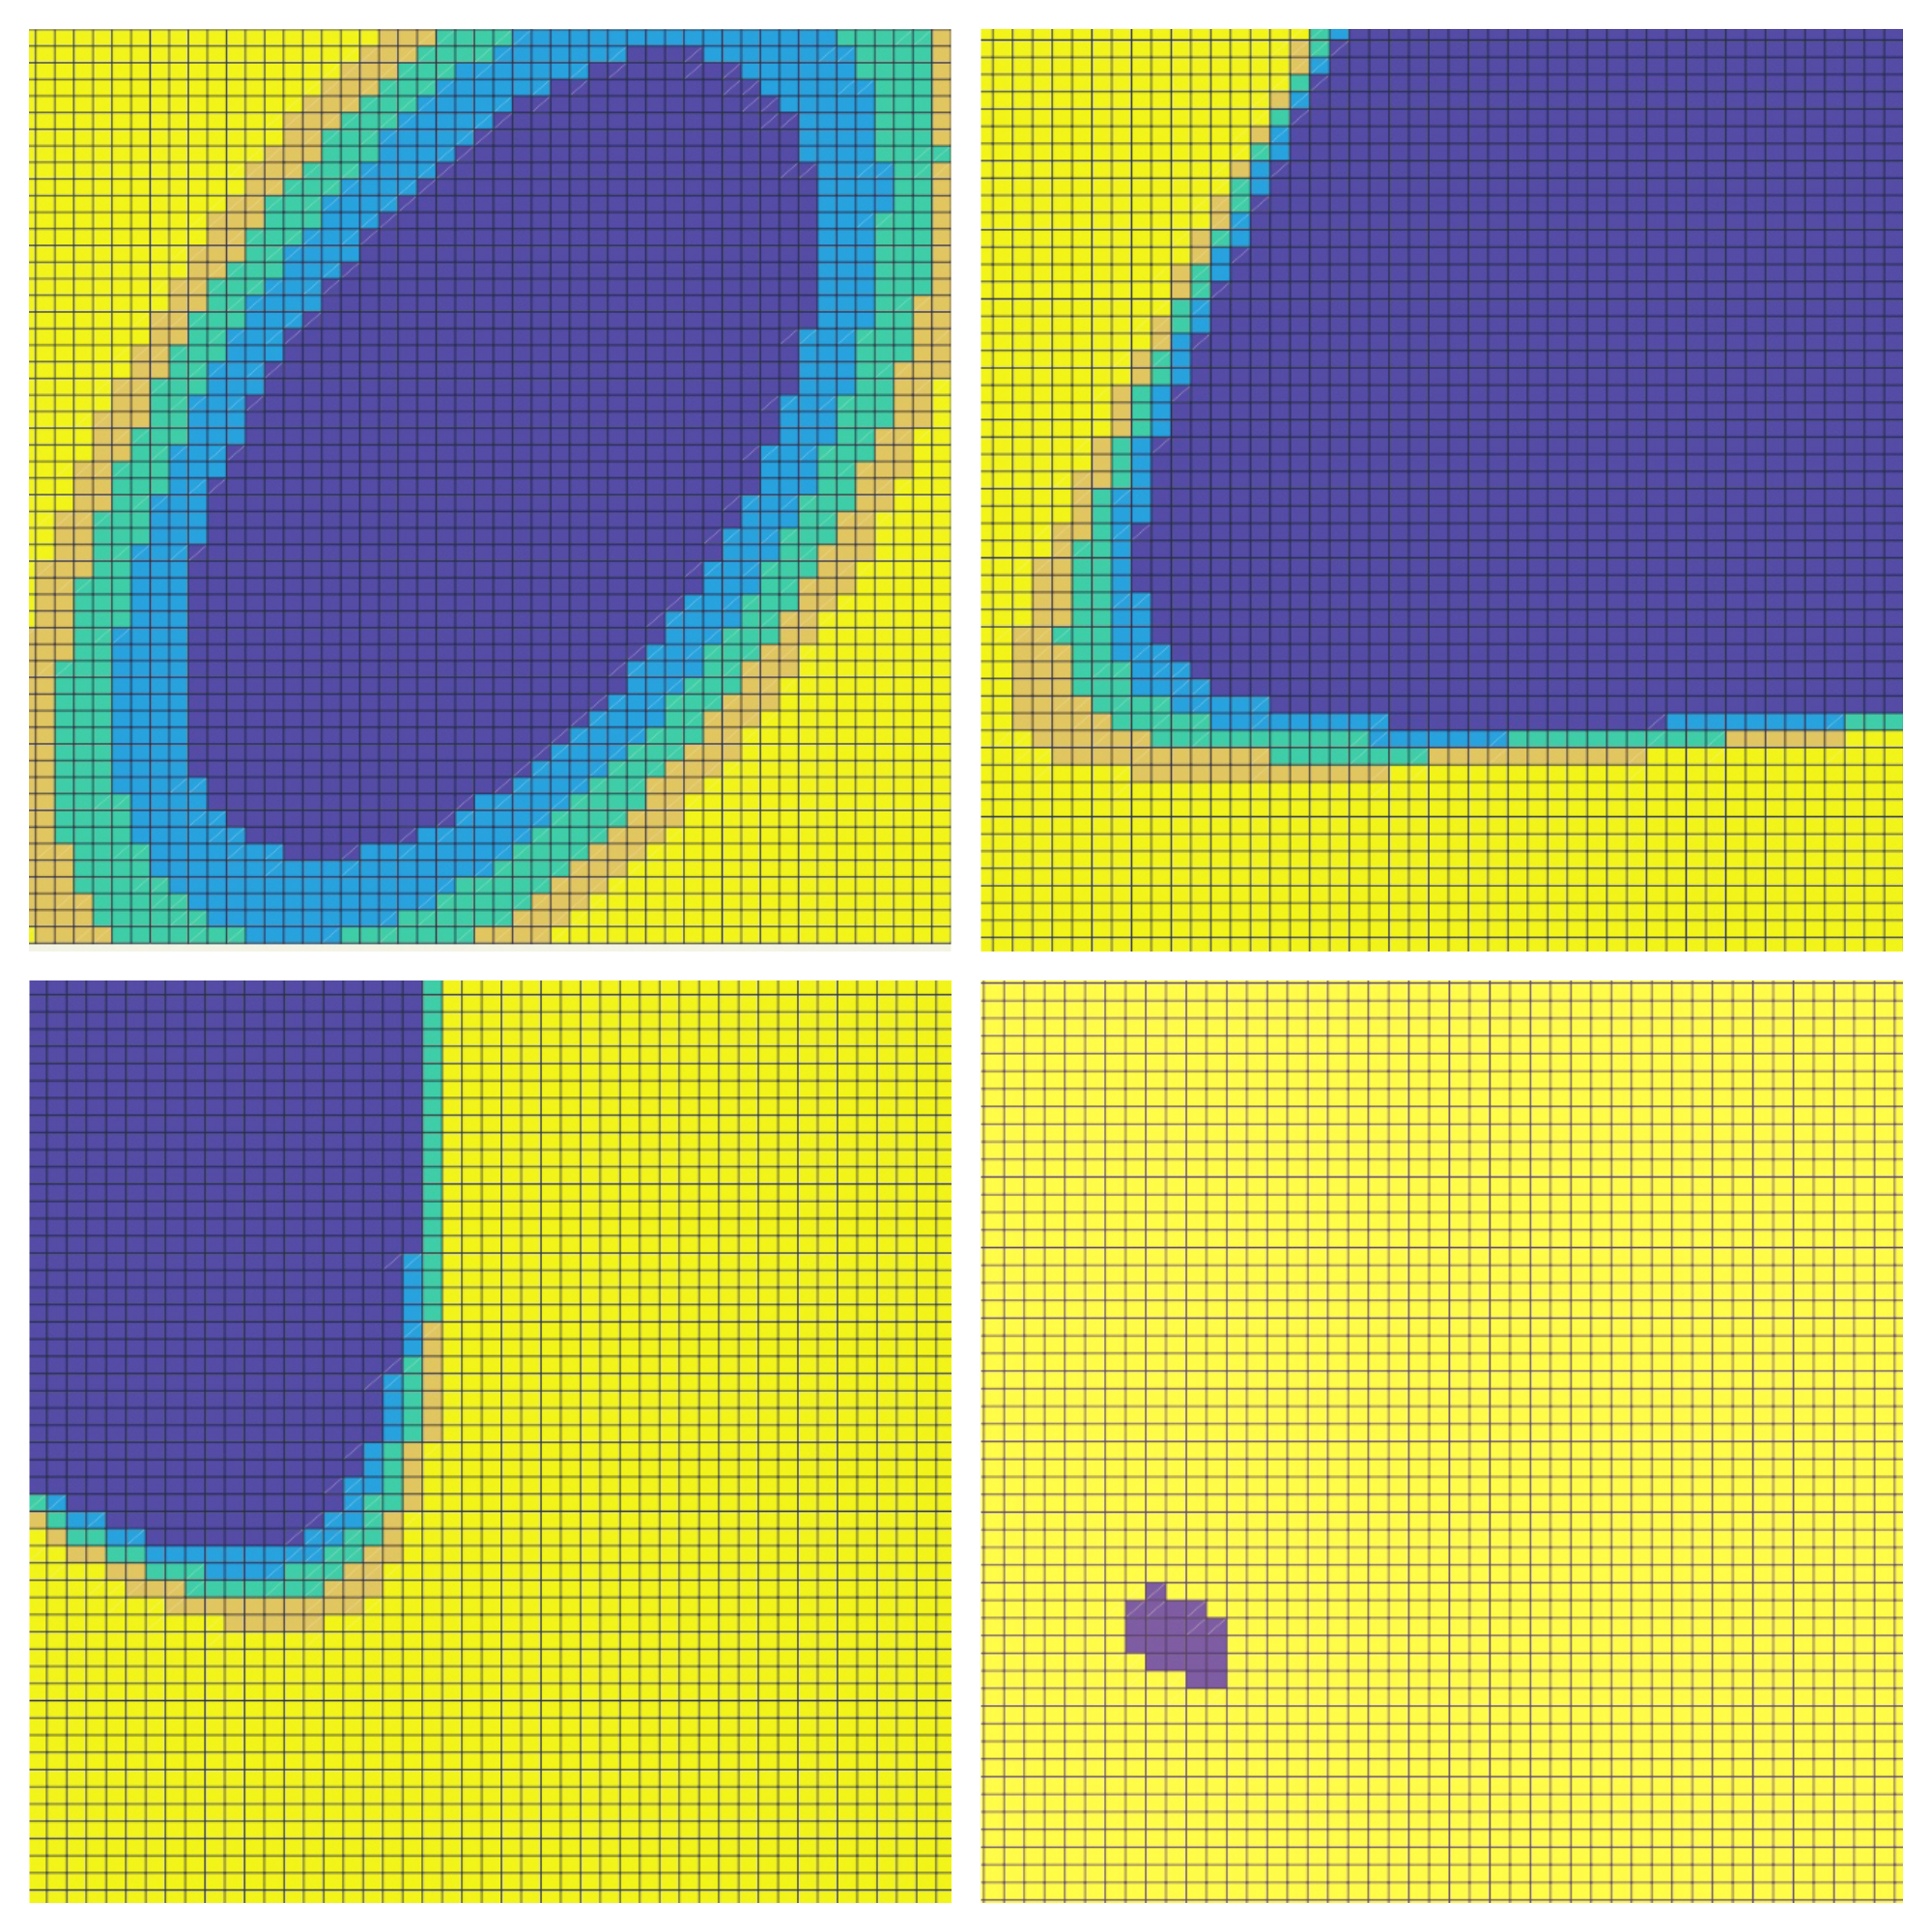
\includegraphics[width=\textwidth,height=\textheight,keepaspectratio]{/Users
/shuping.ruan/Dropbox/Apps/Texpad/Graduate/thesis/Chapter-3/figs/action.jpg}
	\caption{Treatment assignments under four different constraints}
\end{figure}	
\end{minipage}
\end{frame}
%%%%%%%%%%%%%%%%%%%%%%%%%%%%%%%%%%%%%%%%%%%%%%%%%%%%%%%%%%%%%%%%%%%%%%
%\section{Discussion and Future work}
%\subsection{Methodology}
\begin{frame}
	\frametitle{Discussion and Future Work}
	\begin{itemize}
		\item Consistency and asymptotic normality were proven for single-stage and
finite-stage
		\item Theoretical work for infinite-stage constrained problem
		\item Real clinical data application
		\item Incorporate more complex input data, such as omics data, medical
images, etc.
		\item Learning rewards/objective/constraints from clinical experts
	\end{itemize}
\end{frame}
\begin{frame}
\centering
\Large Thank You \& Happy Holidays!	
\end{frame}

%%
%\begin{frame}
%	\frametitle{Learning}
%	Learning constraints \\
%	Learning from medical experts \\
%	Learning automatic rewards generation for medical \\
%	State input, NLP, Vision
%\end{frame}
%
%\subsection{Application}
%\begin{frame}
%	\frametitle{Application}
%	 preventive intervention, behavior change
%\end{frame}
%

\end{document}
